\documentclass[bwprint]{apmcmthesis}

% === Extra packages ===
\usepackage{algorithm2e}
\usepackage{float}
\usepackage{placeins}
\usepackage[hidelinks]{hyperref}
\usepackage{etoolbox}
% 允许最后一行少量拉伸，消除正文右侧 3--10 pt 的溢出
\setlength{\emergencystretch}{6em}
% 类文件默认在节号中插入 \thinspace，标题会显示成“4 . 1”，此处收紧为标准点号
\renewcommand\thesubsection{\arabic{section}.\arabic{subsection}}
\renewcommand\thesubsubsection{\thesubsection.\arabic{subsubsection}}
% 节标题恢复模板的罗马数字（I. II. …），目录条目随 \thesection 自动同步；小节号仍为 4.1 式
\renewcommand{\thesection}{\Roman{section}}
\titleformat{\section}{\centering\normalfont\Large\bfseries}{\thesection.}{.5em}{}
% 目录列到小节（二级），条目用 8.5 pt 正文压缩，使全部 60 条压在一页内
\setcounter{tocdepth}{2}
\titlecontents{section}[0pt]{\bfseries\addvspace{2pt}}{{\thecontentslabel}.\enspace}{}{\titlerule*[0.5pc]{.}\contentspage}
% 引用改为小号上标（原来方括号与正文同字号，显得过大）
\makeatletter
\def\@cite#1#2{\textsuperscript{\scriptsize[#1\if@tempswa , #2\fi]}}
\makeatother
% 摘要页即第 1 页：去掉 \abstract 自带的 \newpage，让标题与摘要同页
\makeatletter
\patchcmd{\abstract}{\newpage}{}{}{}
\makeatother

% 类文件把图表题注设为 \zihao{-4}（12 pt），比正文 10.5 pt 还大；压到 \small
\captionsetup[figure]{font={small,bf}}
\captionsetup[table]{font={small,bf}}
% 收紧浮动体上下间距与题注留白（默认值在 25 图 13 表上会累积出整页空白）
\setlength{\textfloatsep}{10pt plus 2pt minus 2pt}
\setlength{\intextsep}{8pt plus 2pt minus 2pt}
\setlength{\floatsep}{8pt plus 2pt minus 2pt}
\setlength{\abovecaptionskip}{4pt}
\setlength{\belowcaptionskip}{0pt}

% === TikZ ===
\usepackage{tikz}
\usetikzlibrary{arrows.meta,positioning,shapes.geometric,fit,calc}

% === Competition info ===
\tihao{A}
\baominghao{apmcm26300025}
\schoolname{[School Name]}
\membera{[Member A]}
\memberb{[Member B]}
\memberc{[Member C]}

\title{Area-Calibrated SAR--Optical Fusion for Newly Inundated Area Mapping, Probabilistic Intensity Grading and Flood-Cut Relief Allocation in Hengzhou}

\begin{document}

% === Page numbering: the abstract and the contents carry no page number; the body starts at 1 ===
% \thepage prints 1 on the first page after the contents, so the final lastpage label gives
% the body total (47) and the closing page of the appendix reads Page 47 of 47.
\renewcommand{\thepage}{\ifnum\value{page}>2 \the\numexpr\value{page}-2\relax\else\roman{page}\fi}

% === Official template layout: abstract is page 1, title sits above the team table ===
\pagestyle{frontmatterstyle}
\thispagestyle{frontmatterstyle}

\begin{center}
\parbox{0.92\textwidth}{\centering\large\bfseries
Area-Calibrated SAR--Optical Fusion for Newly Inundated Area Mapping,\\[2pt]
Probabilistic Intensity Grading and Flood-Cut Relief Allocation in Hengzhou\par}
\end{center}

\begin{abstract}
\zihao{5}
\noindent\hspace*{2em}Flood relief needs to know where new water stands, whom it reaches and which roads it cuts. This paper reads the \textbf{newly inundated set} $F=W_1\setminus W_0$ from pre-flood optical and post-flood SAR imagery and carries it through a \textbf{five-stage chain}, from recognition to relief allocation in Hengzhou.

The recognizer of Problem~1 starts from the labels: of 65.5 million valid pixels only 2.37\% of the flooded ones were water before the event. Per-tile rank normalization and Lee filtering precede a \textbf{LightGBM} classifier, and spatially blocked five-fold validation gives IoU 0.618 with a total area error of $-0.2\%$ once a 50 px minimum mapping unit is applied (raw 0.598 and $+9.2\%$; split-Otsu $+134\%$). False alarms gather under tree cover, misses in wetland. The mapping unit removes isolated alarms; the baseline's over-detection is connected and survives it.

Problem~2 replaces the pixel classifier with a \textbf{dual-branch gated SAR--optical U-Net} trained on focal, Dice and area-consistency losses: IoU \textbf{0.797} and $+0.9\%$ area error in domain, hard-tile IoU 0.266 to 0.648, and $+1.45\%$ for the modality-dropout variant that carries the model onto SAR-only imagery. Grading reuses that network. Bayes boundaries of a \textbf{Gaussian mixture} on the logit flood share place the four grades at 5.9\%, 53.0\% and 96.9\%; drawing the grade from \textbf{Monte Carlo probabilities} returns 86.2\% correct where LightGBM returns 54.3\%.

Transfer (Problem~3) is where the chain meets unlabelled data. Three Sentinel-1 passes (27 June, 4 July, 16 July 2026) are co-registered to remove a 5.4--6.2\,km offset, and the frozen model runs behind terrain, change and minimum-area guards. On 16 July new inundation is \textbf{26.90\,km$^2$} (0.78\% of the city, grade general); on 4 July, 24.53\,km$^2$. The net increase is $-52.53$\,km$^2$, because the wet-season baseline receded further than the flood advanced.

That raster then ranks 393 settlement catchments on nine overlay indicators (Problem~4; \textbf{entropy--CRITIC--AHP} weights, \textbf{TOPSIS} combination): 13,954 people and 117\,km of road are flooded, Shitang, Maling and Luancheng lead, and the ranking keeps Spearman 0.987 under weight perturbation. A \textbf{location--allocation MILP} on the flood-cut network (Problem~5) opens six depots, reaches 7316 of 13,948 people, and leaves a weighted unmet share of \textbf{0.570} that equals the weighted demand of the 57 cut-off units; the shortfall is geographic, so the share is a floor. Across 600 scenarios CVaR$_{95}$ is 0.651, and the 16 July image lowers the share by 0.039.

Sensitivity tests across the terrain guard, the probability threshold and the water definition leave the grade, the unit ranking and the isolation finding unchanged\cite{deepseek2026,qwen2026,doubao2026}.

\keywords{newly inundated area; SAR--optical gated fusion; area-preserving calibration; Gaussian-mixture intensity grading; location--allocation MILP}
\end{abstract}

\newpage
{\fontsize{9.5}{10.6}\selectfont\lineskiplimit=-\maxdimen\setlength{\baselineskip}{10.6pt}%
\pdfbookmark[1]{\contentsname}{toc}%
{\centering\raisebox{4pt}[0pt][0pt]{\fontsize{15}{18}\selectfont\bfseries\contentsname}\par}%
\vspace{6pt}%
\csname @starttoc\endcsname{toc}}
\newpage

% === Body ===
\pagestyle{mainmatterstyle}
\thispagestyle{mainmatterstyle}
\section[Introduction]{Introduction and Problem Analysis}

\subsection{Background and Task}

A river flood changes the land surface within hours. Emergency managers then have to decide where water now stands that was dry before, how many people and facilities this water reaches, and how relief can still get through a road network that the same water has cut. Synthetic aperture radar (SAR) sees open water through cloud and rain because a smooth water surface reflects the radar pulse away from the sensor and appears dark. Optical imagery taken before the event shows what the land looked like: permanent rivers and ponds, cropland, trees, buildings. The task is a chain of five models built on these two sources.

Problem~1 asks for preprocessing and a recognizer of flood-inundated area on the official Attachment~1 (1000 triplets of pre-flood optical tile, post-flood GF-3 SAR tile and label), evaluated on independent samples with pixel accuracy, the error of newly inundated area, the relative area error and spatial overlap, plus an analysis of false positives (FP) and false negatives (FN) by land cover and of the factors behind area error. Problem~2 asks for a fused, more accurate model whose primary goal is a small area error, and for a four-level intensity grading (general, relatively strong, strong, extremely strong) with explicit area or proportion thresholds and an analysis of how area errors move the grades. Problem~3 transfers the model to the flood around 6 July 2026 in Hengzhou City, Guangxi, and asks for pre-existing water, newly inundated area, net increase, proportion and a map. Problem~4 asks for a regional assessment on self-chosen units with newly inundated area, proportion and intensity as core indicators and with the exposure of people and critical facilities. Problem~5 asks for one rescue optimization fed directly by the image and assessment results, and for a letter to the local emergency authority.

Fig.~\ref{fig:scenario} fixes the scene behind these five questions. A permanent channel runs along the valley floor, a road follows the terrace above it, and the settlements stand on ground that is normally dry. During the event the floor is covered by new water, the road is cut where it dips into the flood, and a terrace settlement can be reached only by boat.

\begin{figure}[!ht]
  \centering
  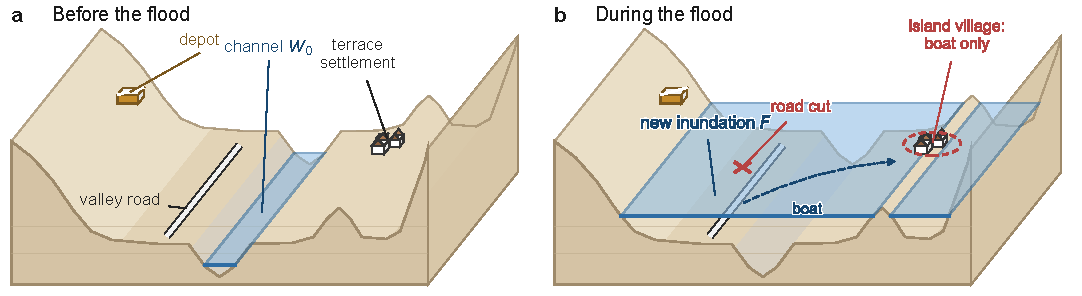
\includegraphics[width=0.90\textwidth,keepaspectratio]{../figures/fig_scenario.pdf}
  \caption{Schematic flood-inundation scenario}
  \label{fig:scenario}
\end{figure}

\subsection{One Definition Shared by All Five Problems}

One chain, one quantity. Because the five problems pass one object from link to link, the definition is fixed here once. We use
\begin{equation}
F=W_1\setminus W_0,\qquad A_{new}=\sum_{p\in F}a_p,\qquad A_{net}=\sum_{p\in W_1}a_p-\sum_{p\in W_0}a_p,\qquad \rho=\frac{A_{new}}{A_{reg}},
\label{eq:def_F}
\end{equation}
where $W_0$ is the water before the flood, $W_1$ the water at the observation time, $a_p$ the true ground area of pixel $p$ and $A_{reg}$ the area of the region or unit. ``Newly inundated area'' is the set $F$ itself; the net increase $A_{net}$ subtracts water that disappeared and can never exceed $A_{new}$ (Section~\ref{sec:data_def}). Two traps follow directly from \eqref{eq:def_F}: counting all post-flood water as new inundation, and reporting the net increase as the new area. Both are avoided by construction.

\subsection{Modeling Route}

Five objects travel along the chain, and Fig.~\ref{fig:roadmap} draws the hand-offs; the arrow labels are those objects, nothing else. From Problem~1 come the baseline recognizer, its FP/FN hotspots by land cover and the hard tiles. A fused model with an area-preserving threshold $\tau_A$ and the grade thresholds $\theta_g$ is what Problem~2 makes of them. Applied unchanged to Sentinel-1 imagery of Hengzhou, that model yields the raster $F$ (Problem~3). Overlaid with population, land cover, roads and facility proxies, $F$ ranks the assessment units of Problem~4; that raster then deletes flooded roads and depots in Problem~5, where the flooded population and index of Problem~4 become demand and priority of a depot-activation and allocation model.

\begin{figure}[!ht]
  \centering
  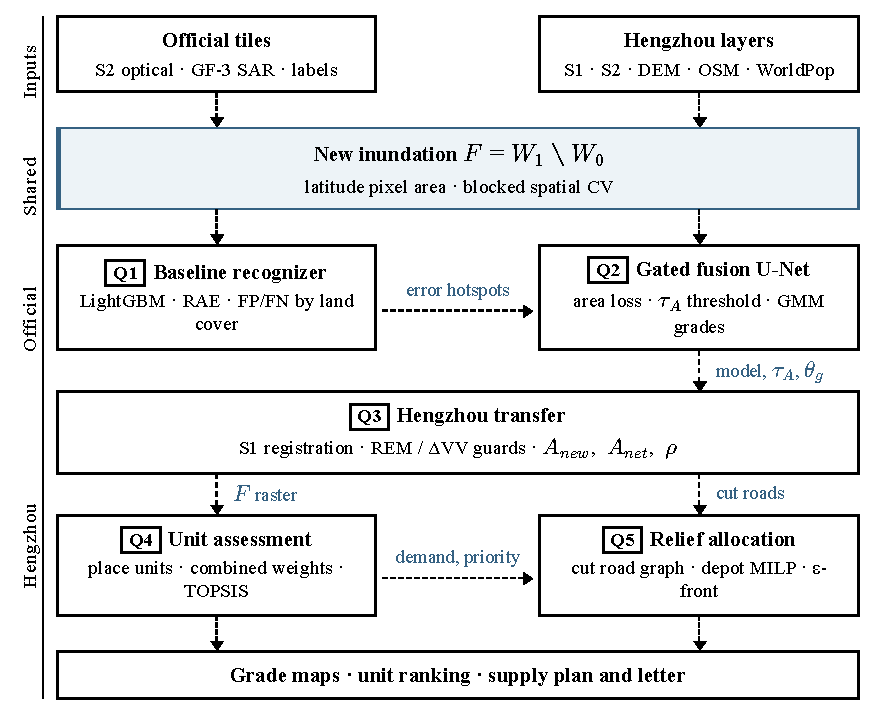
\includegraphics[width=0.82\textwidth,keepaspectratio]{../figures/fig_roadmap.pdf}
  \caption{Technical route of the five-problem chain}
  \label{fig:roadmap}
\end{figure}

Where the two data worlds meet is also drawn in Fig.~\ref{fig:roadmap}. Official tiles occupy the upper half: labels exist there, and every metric can be computed on held-out tiles. The lower half holds only self-collected Hengzhou layers, where no labels exist; there the model output is filtered by physical guards and checked by label-free consistency tests. Training never mixes the two datasets, and exactly three objects cross the boundary: the frozen network weights, the calibration $\tau_A$ and the thresholds $\theta_g$. That separation keeps the Hengzhou numbers of Problems~3--5 traceable to a model whose accuracy was measured on Attachment~1, never tuned towards it.

\subsection{Related Work and What This Paper Adds}

Threshold methods on SAR backscatter remain the operational standard. The split-based rule of Martinis et al.~\cite{martinis2009splitbased} selects bimodal sub-blocks before Otsu's threshold, and automated Sentinel-1 chains add change detection against a reference scene~\cite{twele2016sentinel1}. Deep segmentation networks of the U-Net family~\cite{ronneberger2015unet} trained on labeled Sentinel-1 chips~\cite{bonafilia2020sen1floods11} improve pixel accuracy, but they are usually judged by IoU, not by the area that a disaster report quotes. Terrain descriptors such as the height above the nearest drainage~\cite{nobre2011hand} are commonly used to exclude implausible water on slopes. Relief logistics after a disaster is a facility-location and allocation problem~\cite{balcik2008facility}.

Each choice below answers a gap documented in the cited work, and the first gap is what the recognizer should learn. Testing the official labels on all 65.5 million valid pixels showed that they encode new inundation; the recognizer learns $F$ directly, while Problem~3 still enforces $F\cap W_0=\emptyset$ with an independent $W_0$. Training then targets the area itself. An isotonic probability map followed by an area-preserving threshold makes the mask area equal to the calibrated expected area, and split-conformal intervals attach an error band to every tile. Grade boundaries sit where adjacent components of a Gaussian mixture on the logit flood share are equally likely, with block-bootstrap intervals; a grade becomes a probability vector and not a label alone. The same raster enters the relief model twice, through the cut road graph and through the demand and priority of each unit, and the worth of the second satellite pass becomes the change of the optimal unmet share\cite{deepseek2026,qwen2026,doubao2026}.

\section[Assumptions]{Assumptions and Notation}

\subsection{Model Assumptions}

The following simplifications are needed because the data do not fix them. Each assumed parameter is varied in the sensitivity analyses of the problem where it is used\cite{deepseek2026,qwen2026,doubao2026}.

(1) Tiles of the official dataset inside one block of $5\times5$ tile positions (about $10.4\times11.9$\,km) are spatially dependent, while different blocks are exchangeable. Floods and land cover are autocorrelated over kilometers; random tile or pixel splits would leak information. What makes held-out metrics and conformal intervals meaningful is block-level independence.

(2) The GF-3 uint8 value is a monotone function of radar backscatter whose radiometric scale is unknown. No calibration metadata is supplied; the models see per-tile rank-normalized SAR only, and for Sentinel-1 the scale (dB or amplitude) is chosen by distribution matching.

(3) The Hengzhou flood around 6 July 2026 is represented by the Sentinel-1 passes of 4 July and 16 July, and the pass of 27 June is pre-flood. No pass exists on the reference date. Both flood-time dates are reported and neither is called the peak.

(4) Pre-flood water is the union of independent water sources (pre-flood SAR water, WorldCover water class, OSM water polygons). The union never counts a permanent water pixel as new, so it yields a conservative newly inundated area.

(5) Population is static at the WorldPop 2020 level and uniform inside each 100\,m cell, and every town or city node hosts a township health center that can act as relief depot and facility proxy. No 2026 population grid exists, and OSM lists only five public-service points in the city.

(6) Relief need, depot capacities, fleet and time limits are scenario parameters: 3.5\,kg per person per day (survival water plus ration, Sphere minimum standards) over a 3-day horizon, 60\,t per town depot, 200\,t for the city depot, at most six open depots, 40 trucks of 5\,t and a one-way delivery limit of 120\,min.

\subsection{Notation}

The table collects the symbols that are used across several chapters. Symbols needed only locally are defined where they appear.

\begingroup
\small
\renewcommand{\arraystretch}{0.95}
\begin{longtable}{p{0.16\textwidth}p{0.60\textwidth}p{0.14\textwidth}}
\toprule
Symbol & Meaning & Unit \\
\midrule
\endfirsthead
\toprule
Symbol & Meaning & Unit \\
\midrule
\endhead
\bottomrule
\endfoot
$p$, $t$ & pixel index, tile index & -- \\
$a_p$ & true ground area of pixel $p$ & m$^2$ \\
$z_p$, $\tilde z_p$ & rank-normalized SAR value and its Lee-filtered value & -- \\
$W_0$, $W_1$, $F$ & pre-flood water, flood-time water, newly inundated set $W_1\setminus W_0$ & pixel set \\
$R$ & receded water $W_0\setminus W_1$ & pixel set \\
$A_{new}$, $A_{net}$ & newly inundated area and net increase of inundated area & km$^2$ \\
$A_{reg}$, $\rho$ & area of region or unit; proportion $A_{new}/A_{reg}$ & km$^2$, -- \\
$A_t$, $\hat A_t$, $e_t$ & reference, estimated new area of tile $t$, and $e_t=\hat A_t-A_t$ & km$^2$ \\
RAE, MAE$_A$ & relative total area error; mean absolute tile area error & --, km$^2$ \\
$\bar p_p$ & mean predicted probability of new inundation (MC dropout) & -- \\
$q(\cdot)$, $\tau_A$ & isotonic calibration map; area-preserving threshold & -- \\
$\sigma'_t$, $\mathcal I_t$ & stabilized MC spread of tile area; conformal interval & km$^2$ \\
$\theta_1,\theta_2,\theta_3$ & proportion thresholds of the four intensity grades & -- \\
$\pi_{jg}$ & probability that unit $j$ belongs to grade $g$ & -- \\
$\mathrm{REM}_p$, $h^*$ & relative elevation above nearest drainage; its guard threshold & m \\
$\Delta VV$, $\delta$ & change of VV backscatter against 27 June; change margin & dB \\
$X_{jk}$, $w_k$ & indicator $k$ of unit $j$; indicator weight & mixed, -- \\
$S_j$ & TOPSIS disaster index of unit $j$ & -- \\
$P_j$, $d_j$ & flooded population and relief demand of unit $j$ & persons, t \\
$\eta_i$ & 1 if candidate depot $i$ is opened & -- \\
$x_{ij}$, $u_j$ & relief shipped from depot $i$ to unit $j$; unmet demand of $j$ & t \\
$t_{ij}$, $\mathcal A$ & travel time on the flood-cut network; admissible pairs & min, -- \\
$f_1$, $f_2$ & priority-weighted unmet share; priority-weighted delivery time & --, min \\
\end{longtable}
\endgroup
\addtocounter{table}{-1}% 符号表不占用表号，保证后续表从 1 连续编号

\section[Data and Preprocessing]{Data, Verification and Shared Preprocessing}
\label{sec:data_def}

\subsection{Official Tiles and Self-Collected Layers}

\textbf{Official data (Attachment~1).} Attachment~1 holds 1000 co-registered triplets, IDs 1001--2000: one pre-flood Sentinel-2 tile with four uint8 bands (B, G, R, NIR), one post-flood GF-3 HH SAR tile with a single uint8 band, and a binary label, each $256\times256$ pixels and stored as GeoTIFF in WGS-84 geographic coordinates at $8.333\times10^{-5}$\,degree per pixel. GeoTIFF tags place the tiles between 112.69 and 116.91$^\circ$E and 28.43 and 29.30$^\circ$N, in four spatial clusters of 512, 450, 22 and 16 tiles -- consistent with the Dongting and Poyang lake basins. The attachment states no event date, and we do not assign one. Class imbalance is strong: pixel-weighted, 18.99\% of the labeled pixels are flooded, yet the median tile carries only 3.76\% flood and 15 tiles carry none, which leaves many tiles with almost no target. The README quotes a mean flood share of 24.5\%; a full traversal of the 1000 label files gives 18.99\%, and the verified value is the one used here.

\textbf{Self-collected data (Hengzhou).} Problems~3--5 use only public layers, listed in Table~\ref{tab:hz_data}. They are reprojected to the 10\,m UTM~49N grid of the Sentinel-1 product (nearest neighbor for classes, bilinear for continuous values) and clipped to the GADM~4.1 boundary, whose geodesic area is 3440.09\,km$^2$.

\textbf{Where the layers come from.} The official triplets are the competition attachment (Attachment~1), not an external download. The Hengzhou layers were downloaded from public archives: Sentinel-1 RTC from Microsoft Planetary Computer; Sentinel-2 L2A and the DEM from Copernicus; land cover from ESA WorldCover; OSM extracts from Geofabrik; population from WorldPop; and the boundary from GADM~4.1. Table~\ref{tab:hz_data} gives the date, resolution and use of each layer.

\begin{table}[!ht]
\centering
\caption{Public data used for Hengzhou}
\label{tab:hz_data}
\small
\begin{tabular}{p{0.27\textwidth}p{0.2\textwidth}p{0.15\textwidth}p{0.265\textwidth}}
\toprule
Layer & Date & Resolution & Use \\
\midrule
Sentinel-1 RTC VV/VH (Planetary Computer)\cite{planetary2026} & 27 Jun, 4 Jul, 16 Jul 2026 & 10\,m grid & $W_0$, flood-time water, model input \\
Sentinel-2 L2A (Copernicus)\cite{copernicuss2_2026} & 31 May 2026 & 10\,m & tested, rejected (Sec.~\ref{sec:q3_verify}) \\
ESA WorldCover v200\cite{worldcover2026} & 2021 & 10\,m & $W_0$, land-cover strata, exposure \\
Copernicus DEM GLO-30\cite{copernicusdem_2026} & -- & 30\,m & relative elevation guard \\
OSM roads, water, places (Geofabrik)\cite{geofabrik2026} & 2026 extract & vector & $W_0$, units, road graph \\
WorldPop constrained\cite{worldpop2026} & 2020 & 100\,m & flooded population \\
GADM 4.1 boundary\cite{gadm2026} & -- & vector & study area \\
\bottomrule
\end{tabular}
\end{table}

Fig.~\ref{fig:data_samples} shows only representative samples, not the full inventory. Panels (a)--(c) are one official triplet: pre-flood optical, post-flood SAR and binary label. Panels (d)--(f) are three Hengzhou layers used downstream: Sentinel-1 VV on 16 July, WorldCover, and WorldPop with OSM roads. The Hengzhou panels use a 150\,m display grid. All analyses use their native grids.

\begin{figure}[!ht]
  \centering
  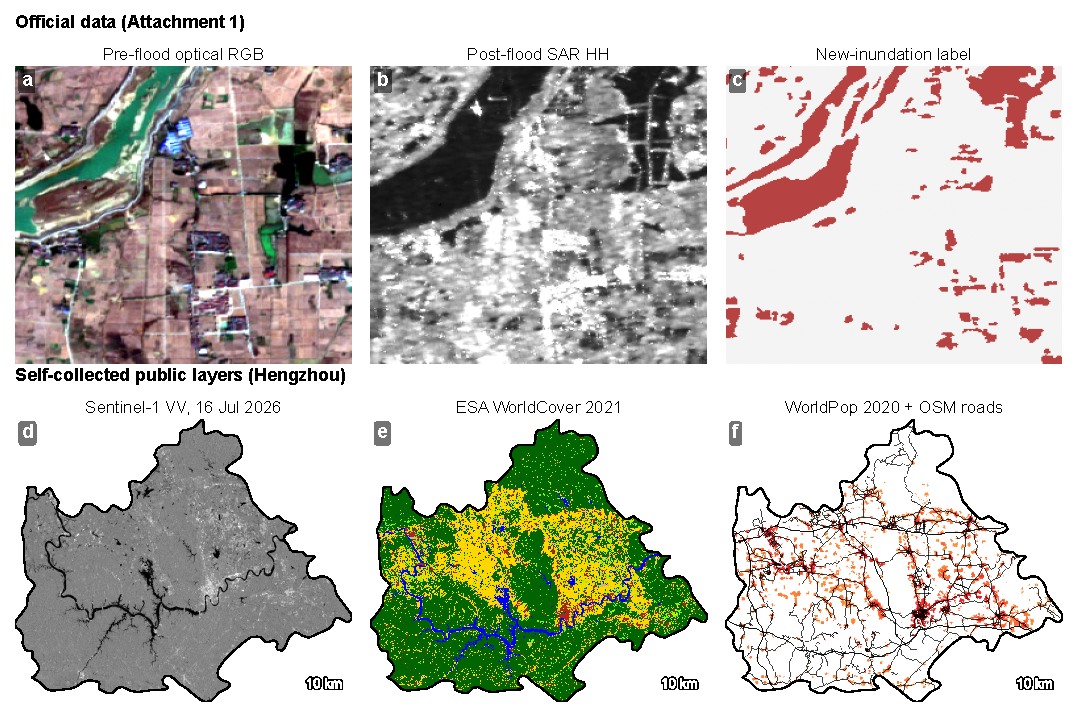
\includegraphics[width=0.90\textwidth,keepaspectratio]{../figures/fig_data_samples.pdf}
  \caption{Representative data samples}
  \label{fig:data_samples}
\end{figure}

Two of its rows needed repair, and the repair belongs to the method. Relative to their geotransform the Sentinel-1 rasters are shifted north--south by 5.4--6.2\,km, and the Sentinel-2 scene cannot be aligned by any translation; both findings, and how they were handled, are reported in Section~\ref{sec:q3_verify}, since they affect only Problems~3--5. Official tiles passed the same test: on the 491 tiles carrying 3--60\% optical water, the shift that best aligns SAR-dark pixels with optical water has a median of $(0,0)$ pixels, and 63.3\% of the tiles align within 2 pixels, which keeps the official triplets on their native grid.

\subsection{What the Official Labels Actually Mark}

The labels are binary and could mean either ``water after the flood'' ($W_1$) or ``new inundation'' ($F$). The difference decides whether a model trained on them learns the quantity the problem asks for. A label that marks $W_1$ must contain the permanent rivers and lakes. A label that marks $F$ must leave them at 0 even though they are dark in the post-flood SAR. We tested this on all 65,491,966 valid pixels with three definitions of pre-flood water ($\mathrm{NDWI}>0$; $\mathrm{NDWI}>0.1$; $\mathrm{NDWI}>0$ and $\mathrm{NDVI}<0$), using the water index of McFeeters~\cite{mcfeeters1996ndwi}.

\begin{figure}[!ht]
  \centering
  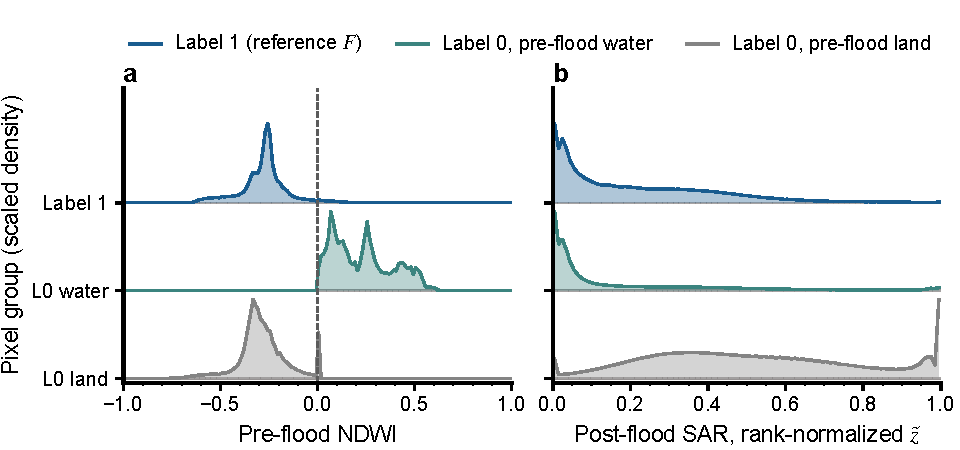
\includegraphics[width=0.90\textwidth,keepaspectratio]{../figures/fig_q1_label_semantics.pdf}
  \caption{Label-semantics test on all valid pixels}
  \label{fig:q1_label_semantics}
\end{figure}

The distributions in Fig.~\ref{fig:q1_label_semantics} separate cleanly. Panel (a) shows pre-flood NDWI for three pixel groups: label-1 pixels sit almost entirely below zero, and only 2.37\% of them had $\mathrm{NDWI}>0$ before the event (2.06\% under the strict definition). Panel (b) shows post-flood SAR brightness: pre-flood water pixels that carry label 0 are just as dark as the flooded pixels, and 70.1\% of them fall below the dark threshold $\tilde z<0.2$. Pre-flood water is therefore still water after the flood, but the labels exclude it. The labels mark newly inundated area with permanent water set to 0, and this holds for all three definitions. Problems~1--2 therefore learn $F$ directly, and Problem~3, where no labels exist, builds $W_0$ independently and subtracts it.

\subsection{Area Definitions and Their Set Logic}

The four sets of \eqref{eq:def_F} are related by $W_1=F\cup(W_0\cap W_1)$ and $W_0=(W_0\cap W_1)\cup R$ with $R=W_0\setminus W_1$, which gives
\begin{equation}
A_{net}=|W_1|_a-|W_0|_a=A_{new}-|R|_a\le A_{new},
\label{eq:net_identity}
\end{equation}
where $|\cdot|_a$ is the area-weighted size of a set. Comparing an estimate $\hat F$ with the reference $F$ splits the area error into false alarms and misses,
\begin{equation}
\hat A-A=|\hat F\setminus F|_a-|F\setminus\hat F|_a=|\mathrm{FP}|_a-|\mathrm{FN}|_a .
\label{eq:fpfn_identity}
\end{equation}
Fig.~\ref{fig:q1_set_logic} draws both identities.

\begin{figure}[!ht]
  \centering
  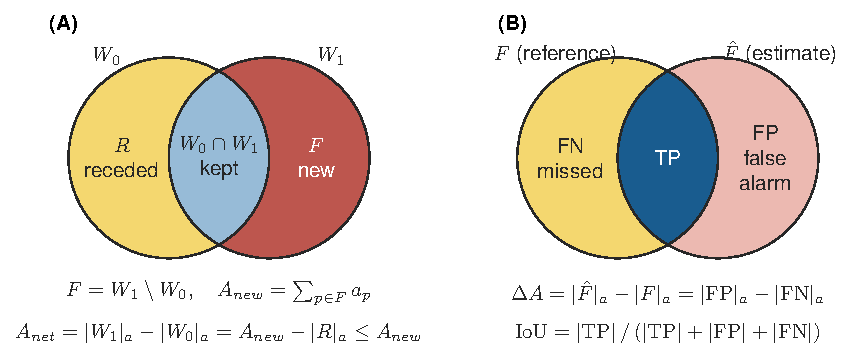
\includegraphics[width=0.90\textwidth,keepaspectratio]{../figures/tikz_q1_set_logic.pdf}
  \caption{Set logic of the area definitions}
  \label{fig:q1_set_logic}
\end{figure}

Panel (a) of Fig.~\ref{fig:q1_set_logic} explains why the net increase can be negative while new inundation is positive: any receded water $R$ (drained ponds, a lower river stage) is subtracted from $A_{new}$, and this happens in Hengzhou. Panel (b) explains why IoU alone is not enough for this problem. Identity \eqref{eq:fpfn_identity} lets a model with many false alarms and as many misses report an almost exact total area. Area error is always reported together with IoU here, split by land cover into FP and FN parts.

\subsection{Shared Preprocessing}

\textbf{Pixel area.} The ground area of a geographic pixel with center latitude $\varphi_p$ and angular sizes $\Delta\lambda,\Delta\varphi$ follows from the WGS-84 meridian and prime-vertical radii, with $a=6378137$\,m and $e^2=0.00669438$:
\begin{equation}
\begin{split}
M(\varphi)&=\frac{a(1-e^2)}{(1-e^2\sin^2\varphi)^{3/2}},\qquad
N(\varphi)=\frac{a}{(1-e^2\sin^2\varphi)^{1/2}},\\
a_p&=M(\varphi_p)\,\Delta\varphi\cdot N(\varphi_p)\cos\varphi_p\,\Delta\lambda .
\end{split}
\label{eq:pixel_area}
\end{equation}
On the official tiles $a_p$ ranges from 74.78 to 75.41\,m$^2$ and the mean tile area is 4.913\,km$^2$. On the Hengzhou UTM grid $a_p=100/k_p^2$\,m$^2$ with the UTM point scale factor $k_p$. Every area in this paper is $\sum a_p$ over a mask.

\textbf{Geometry.} Label, SAR and optical tie points differ by at most 0.47 pixel. Nine label tiles have an anisotropic pixel size ($7.9119\times10^{-5}$ by $8.3349\times10^{-5}$ degree) and are resampled by nearest neighbor onto the SAR grid. Pixels outside the label footprint are excluded from all metrics.

\textbf{SAR normalization and speckle.} The radiometric scale of the GF-3 values is unknown (Assumption~2), and each tile is rank-normalized with its own 2\% and 98\% quantiles,
\begin{equation}
z_p=\mathrm{clip}\!\left(\frac{I_p-Q_2}{Q_{98}-Q_2+\epsilon},0,1\right),\qquad \epsilon=10^{-6},
\label{eq:rank_norm}
\end{equation}
and then filtered by the Lee filter~\cite{lee1980local} on a $5\times5$ window $\Omega_p$:
\begin{equation}
\begin{split}
\tilde z_p&=\bar z_p+k_p\,(z_p-\bar z_p),\qquad
k_p=\max\!\left(0,\ 1-\frac{C_u^2}{C_{z,p}^2}\right),\\
C_{z,p}^2&=\frac{\mathrm{Var}_{\Omega_p}(z)}{\bar z_p^2+\epsilon},\qquad
C_u=\frac{1}{\sqrt L}.
\end{split}
\label{eq:lee}
\end{equation}
The equivalent number of looks $L$ is estimated per tile as the median of $\bar z^2/\mathrm{Var}(z)$ over the 10\% most homogeneous $7\times7$ windows; its median over the official tiles is 31.0. The filter smooths homogeneous areas ($k_p\to0$) and keeps edges ($k_p\to1$), which matters for narrow flooded channels. Because \eqref{eq:rank_norm} uses only the tile itself, no information crosses the validation folds.

\textbf{Optical indices and features.} The validity mask is $m_p=\mathbb 1[\max(B,G,R,N)>0]$; 60 official tiles have more than 5\% invalid optical pixels. From the bands we compute $\mathrm{NDWI}=(G-N)/(G+N+\epsilon)$, $\mathrm{NDVI}=(N-R)/(N+R+\epsilon)$ and the brightness $(B+G+R+N)/1020$. The pixel classifier of Problem~1 uses 19 features: $z$, $\tilde z$, local mean and standard deviation of $\tilde z$ on $3\times3$, $7\times7$ and $15\times15$ windows, the $7\times7$ minimum of $\tilde z$, the three indices and the $7\times7$ mean NDWI, the four scaled bands, $m_p$, and the interaction $\tilde z(1-\mathrm{NDWI}^+)$, which encodes ``dark now and not water before''\cite{deepseek2026,qwen2026,doubao2026}.

\section[Problem 1]{Problem 1: Area-Oriented Recognition of Newly Inundated Area}
\label{sec:q1}

\subsection{Independent Samples by Spatially Blocked Cross-Validation}

The problem asks for evaluation ``using independent samples''. Neighbouring tiles share the same flood and the same fields, so a random split of tiles, let alone of pixels, would put near-copies of a test tile into training. The 1000 tiles lie on a regular grid of $199\times42$ tile positions. We group them into 67 blocks of $5\times5$ positions (Assumption~1) and assign the blocks to five folds by a greedy stratified rule that balances tile count and flood area. For outer fold $k=0,\dots,4$,
\begin{equation}
\begin{split}
\mathcal T^{test}_k&=\mathcal F_k,\\
\mathcal T^{cal}_k&=\mathcal F_{(k+1)\bmod 5},\\
\mathcal T^{train}_k&=\Big\{t\notin\mathcal F_k\cup\mathcal F_{k+1}:\ \min_{s\in\mathcal F_k\cup\mathcal F_{k+1}}\lVert g_t-g_s\rVert_\infty>1\Big\},
\end{split}
\label{eq:folds}
\end{equation}
where $\mathcal F_k$ is the set of tiles in fold $k$ and $g_t$ the grid position of tile $t$. The calibration fold is used for every choice that would otherwise peek at the test data (threshold, early stopping, isotonic map, conformal quantile), and the Chebyshev buffer of one tile removes the training tiles that touch a test or calibration tile. The resulting test folds hold 194, 200, 202, 202 and 202 tiles with flood shares 0.184--0.202, and 170--196 buffer tiles are dropped from each training set. Every tile is tested exactly once, so all metrics below are pooled over the 1000 held-out tiles. This design follows the recommendation of blocked cross-validation for spatially structured data~\cite{roberts2017crossvalidation}.

\subsection{Two Recognizers of Different Kinds}

\textbf{Baseline A: physics two-stage rule.} The classical route estimates post-flood water from SAR and subtracts pre-flood water from optics. Each tile is cut into 16 sub-blocks of $64\times64$ pixels, and Otsu's threshold $\tau_b$ on $\tilde z$ is accepted for a sub-block only if its two classes are clearly bimodal~\cite{martinis2009splitbased},
\begin{equation}
D_b=\frac{\sqrt2\,|\mu_1-\mu_2|}{\sqrt{s_1^2+s_2^2}}>2\quad\text{and}\quad \min(n_1,n_2)\ge0.1\,(n_1+n_2),
\label{eq:ashman}
\end{equation}
where $\mu_i,s_i,n_i$ are the class means, standard deviations and sizes (Ashman's $D$). The tile threshold is the median of the accepted $\tau_b$, with a fold-level median as fallback. Then $\hat F_A=\{\tilde z<\tau\}\setminus\{\mathrm{NDWI}>0\}$, and components smaller than 10 pixels are removed. Labels are not used at all, so baseline A measures how far a rule without training gets.

\textbf{Baseline B: LightGBM pixel classifier.} The second recognizer learns $\Pr(y_p=1\mid\boldsymbol x_p)$ from the 19 features of Section~\ref{sec:data_def} with gradient-boosted trees~\cite{lightgbm2020package}. Because labels mark new inundation, the classifier learns $F$ directly. Up to 2000 pixels per training tile are drawn, half positive and half negative where possible (about 0.8\,M rows per fold), which handles the imbalance; the prior shift this causes is absorbed by the threshold
\begin{equation}
\tau_k=\arg\max_{\tau\in\{0.05,0.06,\dots,0.95\}}\ \mathrm{F1}\big(\mathcal T^{cal}_k;\tau\big),
\label{eq:tau_f1}
\end{equation}
chosen on the calibration fold. The trees use 63 leaves, learning rate 0.05 and early stopping after 50 rounds on calibration pixels; the selected thresholds were 0.46, 0.58, 0.77, 0.40 and 0.59 with 390--1211 trees.

\subsection{Pixel and Area Metrics}

Pixel metrics (overall accuracy OA, precision, recall, F1, IoU and Cohen's $\kappa$) come from the pooled confusion matrix. The area metrics follow the problem's emphasis and use the tile error $e_t=\hat A_t-A_t$ with $A_t=\sum_{p\in t}a_py_p$:
\begin{equation}
\begin{split}
\Delta A&=\sum_te_t,\qquad
\mathrm{RAE}=\frac{\sum_t\hat A_t-\sum_tA_t}{\sum_tA_t},\\
\mathrm{MAE}_A&=\frac1T\sum_t|e_t|,\qquad
\mathrm{RAE}_t=\frac{e_t}{A_t}\ \ (A_t\ge0.05\ \mathrm{km}^2).
\end{split}
\label{eq:area_metrics}
\end{equation}
RAE measures bias of the total, while MAE$_A$ measures how wrong a single tile is; the two differ because tile errors of opposite sign cancel in $\Delta A$ (identity \eqref{eq:fpfn_identity}). The floor of 0.05\,km$^2$ (about 1\% of a tile) avoids dividing by near-zero reference areas. Agreement is also shown by the Bland--Altman bias $\bar e$ and limits $\bar e\pm1.96s_e$~\cite{bland1986agreement}.

\subsection{Recognition Results on 1000 Held-out Tiles}

Table~\ref{tab:q1_metrics} gives the pooled results. The two baselines differ by a factor of more than two in IoU and by a factor of 15 in total area bias.

\begin{table}[H]
\centering
\caption{Held-out performance of the Problem 1 recognizers}
\label{tab:q1_metrics}
\resizebox{\textwidth}{!}{%
\begin{tabular}{lccccccccc}
\toprule
Model & OA & Precision & Recall & F1 & IoU & $\kappa$ & RAE & MAE$_A$ (km$^2$) & median $|\mathrm{RAE}_t|$ \\
\midrule
A: split-Otsu $-$ NDWI & 0.634 & 0.308 & 0.740 & 0.435 & 0.278 & 0.227 & $+1.406$ & 1.756 & 2.84 \\
B: LightGBM (M0) & 0.900 & 0.717 & 0.783 & 0.749 & 0.598 & 0.686 & $+0.092$ & 0.430 & 0.52 \\
\bottomrule
\end{tabular}}
\end{table}

The 1000 reference tiles contain 933.41\,km$^2$ of new inundation. LightGBM returns 1019.12\,km$^2$, 9.2\% above the reference (an excess of 85.71\,km$^2$). Its fold-level RAE ranges from $-13.9\%$ to $+34.6\%$ (IoU 0.546--0.622), so the pooled value hides a spread that a single random split would never show. Baseline A finds 74\% of the flooded pixels but also labels 2245.66\,km$^2$ as new water, 2.4 times the reference. The reason is visible in its own diagnostic: the Ashman test of \eqref{eq:ashman} passes on 92\% of the sub-blocks, also on tiles without water, because dark fields and bright villages form a bimodal histogram too. We report this as a finding about the baseline and did not tune it on the test labels.

The pooled numbers do not tell where on a tile the errors occur. Fig.~\ref{fig:q1_visual_cmp} therefore shows four held-out tiles of increasing flood share, each predicted by the model of the fold in which it was a test tile; columns 4--6 are confusion maps (true positives, FP, FN) of baseline A, LightGBM and the final Problem~2 model M6.

\begin{figure}[H]
  \centering
  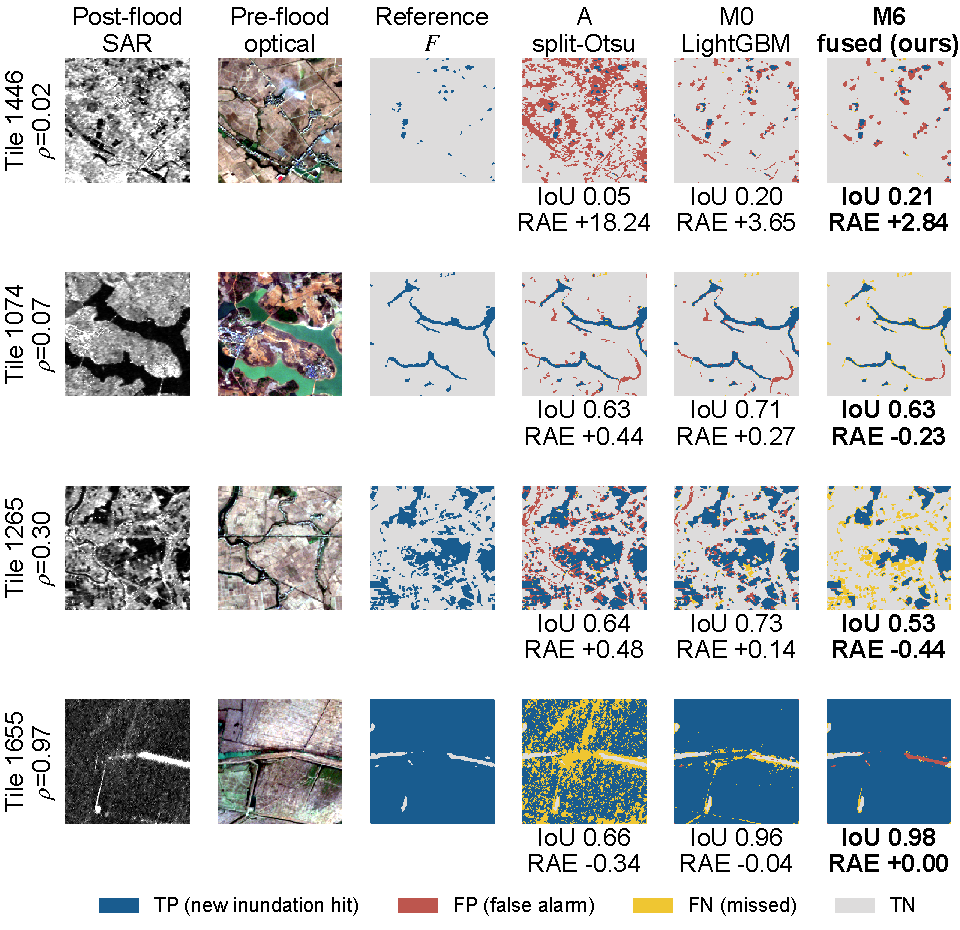
\includegraphics[width=0.98\textwidth,keepaspectratio]{../figures/fig_q1_visual_cmp.pdf}
  \caption{Held-out predictions on four official tiles}
  \label{fig:q1_visual_cmp}
\end{figure}

On tile 1446, where only 1.8\% of the area is flooded, every method fails in the same way: baseline A reaches IoU 0.052 with a relative area error of $+18.2$, and LightGBM still predicts 4.65 times the reference area (RAE$_t=+3.65$), because a few dark fields form most of the prediction. On the medium tiles 1074 ($\rho=7.4\%$) and 1265 ($\rho=30.5\%$) LightGBM has IoU 0.707 and 0.734 and area errors of $+27\%$ and $+15\%$; the false alarms sit along field edges and the misses inside vegetated patches. On the almost fully flooded tile 1655 ($\rho=97.3\%$) LightGBM reaches IoU 0.959 and M6 0.980 with an area error of $+0.4\%$. Relative area error is therefore driven by small reference areas, not by poor pixel classification, which is why the per-tile error has to be read together with the total.

Every held-out tile is also exported as a mask, and Fig.~\ref{fig:q1_pred_set} shows five of them that do not appear in Fig.~\ref{fig:q1_visual_cmp}, spanning a reference share from 2\% to 94\%. At the almost dry tile 1720 baseline A labels half of the tile as water, while LightGBM stays at 5.2\%; at the flooded tiles both follow the water outline.

\begin{figure}[H]
  \centering
  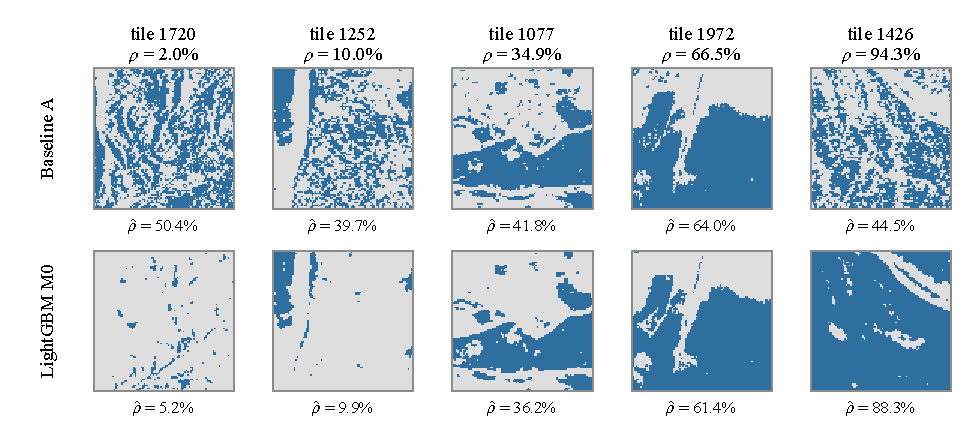
\includegraphics[width=0.95\textwidth,keepaspectratio]{../figures/fig_q1_pred_examples.pdf}
  \caption{Exported tile masks: baseline A (top) and LightGBM M0 (bottom), new water in blue}
  \label{fig:q1_pred_set}
\end{figure}

That observation becomes quantitative in the Bland--Altman plot of Fig.~\ref{fig:q1_area_agreement}, which compares estimated and reference tile areas for all 1000 tiles.

\begin{figure}[H]
  \centering
  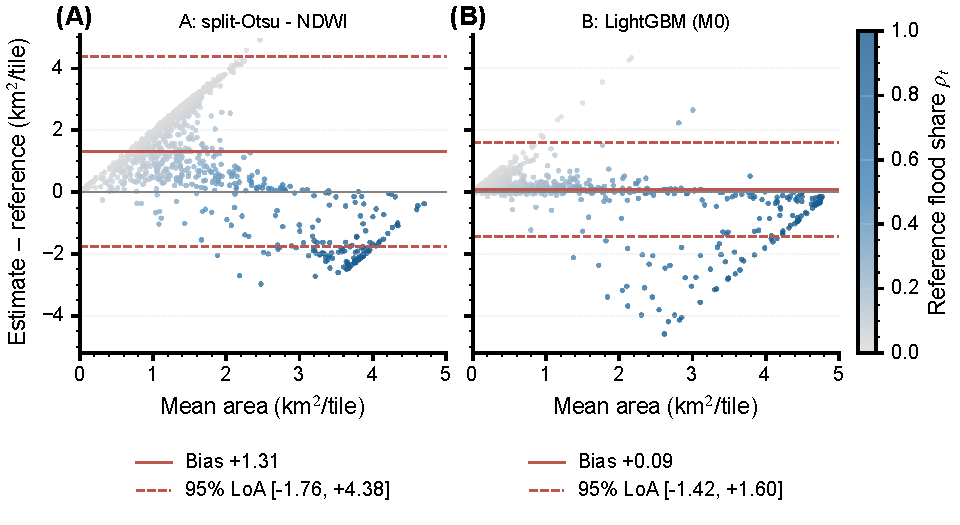
\includegraphics[width=0.95\textwidth,keepaspectratio]{../figures/fig_q1_area_agreement.pdf}
  \caption{Bland--Altman agreement of tile new-inundation area}
  \label{fig:q1_area_agreement}
\end{figure}

Baseline A over-estimates by $+1.31$\,km$^2$ per tile on average, with 95\% limits of $-1.76$ to $+4.38$\,km$^2$, and the excess grows on tiles with little reference flood (panel a). LightGBM removes most of the bias ($+0.086$\,km$^2$) but its limits of agreement, $-1.42$ to $+1.60$\,km$^2$, are still wide compared with the mean tile area of 4.91\,km$^2$. The scatter is widest on tiles with intermediate flood share, where fragmented flood patches meet dark fields. A model whose area error has to be small on each assessment unit, not only in the city total, therefore needs spatial context, which motivates the convolutional model of Problem~2.

\subsection{False Positives and False Negatives by Land Cover}

The problem asks how FP and FN under different land covers affect the area. With land-cover stratum $c$, identity \eqref{eq:fpfn_identity} decomposes exactly:
\begin{equation}
\mathrm{FP}_c=\sum_{p\in c}a_p\hat y_p(1-y_p),\qquad
\mathrm{FN}_c=\sum_{p\in c}a_p(1-\hat y_p)y_p,\qquad
\Delta A=\sum_c(\mathrm{FP}_c-\mathrm{FN}_c).
\label{eq:fpfn_strata}
\end{equation}
The attachment carries no land cover, so the strata come from ESA WorldCover 2021, read for each tile footprint and resampled by nearest neighbour; this describes the pre-flood land state under the assumption that it did not change much between 2021 and the image date. Table~\ref{tab:q1_fpfn} lists the decomposition for LightGBM.

\begin{table}[H]
\centering
\caption{Area decomposition of LightGBM errors by pre-flood land cover (km$^2$)}
\label{tab:q1_fpfn}
\begin{tabular}{lcccc}
\toprule
Stratum & Reference $F$ & FP & FN & Net FP$-$FN \\
\midrule
Tree & 33.46 & 79.80 & 4.93 & $+74.87$ \\
Shrub / grassland & 53.92 & 23.43 & 7.65 & $+15.77$ \\
Cropland & 379.62 & 105.59 & 59.09 & $+46.50$ \\
Built-up & 8.79 & 19.38 & 1.81 & $+17.57$ \\
Bare & 7.97 & 7.70 & 1.15 & $+6.54$ \\
Permanent water & 156.06 & 26.80 & 50.91 & $-24.11$ \\
Wetland & 293.59 & 25.46 & 76.89 & $-51.43$ \\
\bottomrule
\end{tabular}
\end{table}

The table shows two opposite mechanisms. On dry land covers the model raises false alarms: tree cover contributes 79.80\,km$^2$ of FP against only 33.46\,km$^2$ of real new flood, built-up land 19.38\,km$^2$ against 8.79\,km$^2$. Radar shadow behind tree canopies and smooth surfaces in villages look as dark as water. On wet land covers it misses flood: in wetland and areas that WorldCover maps as permanent water, the net error is $-51.43$ and $-24.11$\,km$^2$, because water that rose over a wetland or a lake margin is hard to tell from the water that was already there. The positive and negative nets cancel to the total $+85.71$\,km$^2$; the worst strata by absolute net error are tree, wetland and cropland.

\subsection{Key Factors of Area Accuracy}

To find the factors behind the tile error, each held-out tile gets label-free descriptors (raw SAR mean and standard deviation, share of bimodal sub-blocks, ENL, mean NDVI, WorldCover shares, optical invalid share) together with the reference flood share and the boundary density of the reference flood (perimeter over area). A gradient-boosted regressor on the same spatial folds predicts $|e_t|$ from these descriptors (out-of-fold $R^2=0.417$), and TreeSHAP values~\cite{lundberg2020trees} rank the factors. Fig.~\ref{fig:q1_error_drivers} combines this ranking with the land-cover decomposition.

\begin{figure}[H]
  \centering
  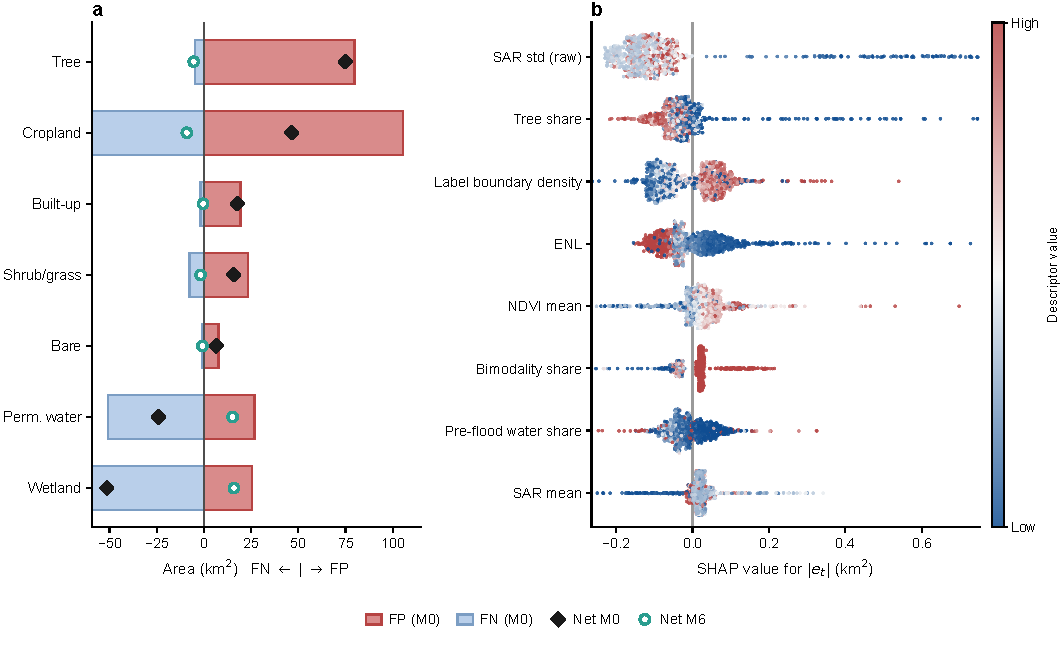
\includegraphics[width=0.98\textwidth,keepaspectratio]{../figures/fig_q1_error_drivers.pdf}
  \caption{Error structure of the Problem 1 model}
  \label{fig:q1_error_drivers}
\end{figure}

Panel (a) of Fig.~\ref{fig:q1_error_drivers} repeats the FP/FN bars of Table~\ref{tab:q1_fpfn} and adds the net error of the Problem~2 model M6 for later comparison. Panel (b) ranks the drivers of absolute tile error by mean $|\mathrm{SHAP}|$: the raw SAR standard deviation is first (0.196), followed by tree share (0.077), boundary density of the flood (0.074), ENL (0.073), NDVI mean (0.057), bimodality share (0.050) and pre-flood water share (0.045). High SAR variance and low ENL mean strong speckle and mixed scattering, tree share is the FP mechanism of Table~\ref{tab:q1_fpfn}, and a high boundary density means fragmented flood that a pixel classifier cuts into pieces. For the signed error the reference flood share comes first, i.e. the model over-estimates on lightly flooded tiles and under-estimates on heavily flooded ones.

A harder notion of independence holds out a whole spatial cluster. Training on three of the four clusters and testing on the fourth lowers the pooled IoU from 0.598 to 0.508 and F1 from 0.749 to 0.674, and the cluster RAE is $+26\%$ on the 512-tile cluster and $+15\%$ on the 450-tile cluster. Transfer to an unseen region thus costs about 0.09 IoU and adds a positive area bias, which is what Problem~3 has to face in Guangxi.

These analyses define what Problem~2 must fix. The 397 tiles with $A_t\ge0.05$\,km$^2$ and $|\mathrm{RAE}_t|>0.5$ under LightGBM form the ``hard set''. The dominant error mechanisms are dark dry surfaces (tree, built-up) and fragmented or vegetated flood, both of which need spatial context and the optical land state, and the dominant error measure is a positive total bias that pixel-wise training does not control.

\section[Problem 2]{Problem 2: Gated SAR--Optical Fusion with Area Calibration and Probabilistic Grading}
\label{sec:q2}

\subsection{Inherited Settings and New Components}

Nothing in Problem~2 starts from zero. The preprocessing, the folds \eqref{eq:folds}, the metrics \eqref{eq:area_metrics} and the land-cover strata carry over from Problem~1 unchanged; every number below can be read against Table~\ref{tab:q1_metrics} on the same 1000 held-out tiles (all variants share one test-tile hash). What changes answers the four diagnoses of Section~\ref{sec:q1}, one component each. Fragmented flood and isolated dark surfaces need spatial context, which a pixel classifier does not have; the classifier gives way to a convolutional network. Dark fields and permanent ponds need the pre-flood optical state, which enters through gated feature fusion. An area-aware loss during training, followed by an area calibration, answers the positive total bias. Tile-level intervals carry the uncertainty into the grading, where it has to survive the transfer. Hengzhou adds a fifth requirement no component above provides: the model must run when the optical input is missing.

\subsection{Dual-Branch Gated Fusion Network}

Two U-Net encoders~\cite{ronneberger2015unet} form the network. The SAR branch reads $[z,\tilde z,\mathrm{std}_7(\tilde z)]$; the optical branch reads $[B,G,R,N]/255$, NDWI, NDVI and the validity $m_p$. Four stages of width 16, 32, 64 and 128 make up each branch (two $3\times3$ convolutions with batch normalization and ReLU, then $2\times2$ max-pooling). At every scale $s$ a learned gate mixes the two feature maps $h_S^{(s)}$ and $h_O^{(s)}$,
\begin{equation}
g^{(s)}=\sigma\!\left(W_g^{(s)}*\big[h_S^{(s)};h_O^{(s)}\big]\right),\qquad
h^{(s)}=g^{(s)}\odot h_S^{(s)}+\big(1-g^{(s)}\big)\odot h_O^{(s)},
\label{eq:gate}
\end{equation}
where $W_g^{(s)}$ is a $1\times1$ convolution, $\sigma$ the logistic function and $\odot$ the element-wise product. The fused map feeds the skip connection of a U-Net decoder (bottleneck 256 channels, bilinear upsampling, dropout 0.2), which ends in a $1\times1$ convolution to the logit $o_p$. Parameters number 2.30\,M, and Fig.~\ref{fig:arch_fusion} shows the data flow.

\begin{figure}[!ht]
  \centering
  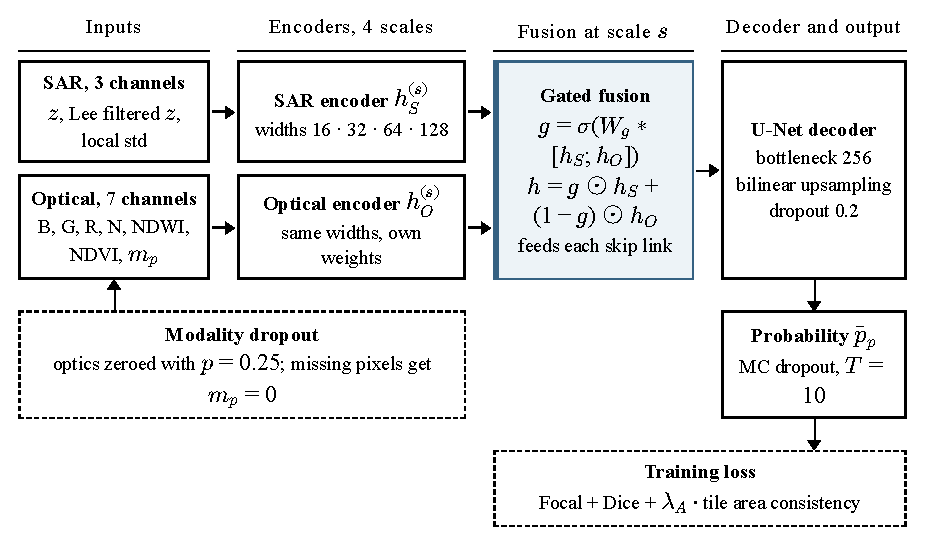
\includegraphics[width=0.90\textwidth,keepaspectratio]{../figures/fig_arch_fusion.pdf}
  \caption{Dual-branch gated fusion network}
  \label{fig:arch_fusion}
\end{figure}

Per pixel and per channel, the gate of \eqref{eq:gate} decides how much to trust each sensor. Where the optical image says ``river before the flood'', the gate can lean on optics to suppress a SAR-dark pixel; where optics are cloudy, it can lean on SAR. Weight is distributed almost evenly: mean SAR gate values are 0.52, 0.57, 0.56 and 0.53 at the four scales, and neither sensor is ignored. A modality-dropout block at the bottom of Fig.~\ref{fig:arch_fusion} sets the entire optical input and $m_p$ to zero with probability 0.25 per training sample, and invalid optical pixels are always zeroed. Working from SAR alone where optics are missing is part of what the model learns; Hengzhou is exactly that case (Section~\ref{sec:q3}).

\textbf{Area-consistent loss.} With $\hat p_p=\sigma(o_p)$, $\hat p_{p,y}$ the probability of the true class, batch $\mathcal B$ and $N_b$ valid pixels in sample $b$, training minimizes
\begin{equation}
\mathcal L=-\frac{1}{|\mathcal V|}\sum_p\alpha_y(1-\hat p_{p,y})^{\gamma}\log\hat p_{p,y}
+\left(1-\frac{2\sum_p\hat p_py_p+1}{\sum_p\hat p_p+\sum_py_p+1}\right)
+\frac{\lambda_A}{|\mathcal B|}\sum_{b\in\mathcal B}\frac{\big|\sum_{p\in b}(\hat p_p-y_p)\big|}{N_b},
\label{eq:loss}
\end{equation}
a focal term~\cite{lin2017focal} ($\gamma=2$, $\alpha_1=0.75$) against the imbalance, a Dice term against the dominance of empty pixels, and an area-consistency term that penalizes the difference between the expected and the true flood area of each tile. Training uses Adam with learning rate $10^{-3}$ and cosine decay, batch 16, flips and $90^\circ$ rotations, at most 40 epochs, and early stopping on the calibration-fold MAE$_A$ with patience 8.

\subsection{Turning Probabilities into an Unbiased Area}

A segmentation threshold of 0.5 maximizes neither accuracy nor area agreement. We therefore calibrate on the calibration fold in three steps.

\textbf{(i) Ensemble mean.} With dropout active at inference, $T=10$ stochastic forward passes give $\bar p_p=\frac1T\sum_{\ell}\hat p_p^{(\ell)}$.

\textbf{(ii) Isotonic calibration.} A monotone map $q$ estimates $\Pr(y=1\mid\bar p)$~\cite{zadrozny2002calibration}:
\begin{equation}
q=\arg\min_{q\ \text{non-decreasing}}\ \sum_{p\in\mathrm{cal}}\big(y_p-q(\bar p_p)\big)^2 .
\label{eq:isotonic}
\end{equation}

\textbf{(iii) Area-preserving threshold.} $\tau_A$ is chosen so that the area of the binary mask equals the calibrated expected area:
\begin{equation}
\sum_{p\in\mathrm{cal}}a_p\,\mathbb 1\big[\bar p_p\ge\tau_A\big]=\sum_{p\in\mathrm{cal}}a_p\,q(\bar p_p).
\label{eq:tauA}
\end{equation}
The left side is non-increasing in $\tau_A$, the right side is constant, and bisection on $[0.01,0.99]$ with tolerance $10^{-4}$ finds the solution. The final mask is $\hat F=\{\bar p\ge\tau_A\}$, and the reported area is the area of that mask; maps and areas agree by construction. Fold thresholds were $\tau_A=0.708$, 0.515, 0.388, 0.690 and 0.574. Calibration folds give a mask area of 933.111\,km$^2$ against an expected 933.112\,km$^2$, a relative gap of $6\times10^{-7}$. On calibration data the identity holds exactly; on test data the remaining bias is an empirical result.

\textbf{Tile intervals.} The MC spread of the tile area, $\sigma_t=\mathrm{std}_\ell\big(\sum_{p\in t}a_p\mathbb 1[\hat p^{(\ell)}_p\ge\tau_A]\big)$, is stabilized as $\sigma'_t=\sigma_t+c$ with $c$ the larger of the calibration median of $\sigma_t$ and 0.005\,km$^2$. Split-conformal prediction~\cite{lei2018conformal} then gives a distribution-free tile interval:
\begin{equation}
\begin{split}
s_t&=\frac{|A_t-\hat A_t|}{\sigma'_t},\qquad
\hat q=s_{(\lceil(n+1)(1-\alpha)\rceil)},\\
\mathcal I_t&=\Big[\max(0,\ \hat A_t-\hat q\sigma'_t),\ \min(A^{tile}_t,\ \hat A_t+\hat q\sigma'_t)\Big],
\end{split}
\label{eq:conformal}
\end{equation}
with $\alpha=0.1$, scores $s_t$ from the $n\approx200$ calibration tiles of the fold, and $A^{tile}_t$ the tile area. The signed standardized residuals $r_t=(A_t-\hat A_t)/\sigma'_t$ of all calibration folds form the residual pool $\mathcal R$ used for the grade uncertainty below.

\subsection{Ablation: Which Component Reduces the Area Error}

Seven trained variants share a held-out set: M0 is the Problem~1 LightGBM; M1 a SAR-only U-Net (focal and Dice loss); M2 adds the gated optical branch; M3 an area term ($\lambda_A=1$); M4 modality dropout and the validity channel; M5 the MC-dropout mean; M6 isotonic calibration and $\tau_A$. The two MMU rows apply 50 px post-processing to M2 and M6 and are not ablation steps. Table~\ref{tab:q2_ablation} lists the metrics.

\begin{table}[!ht]
\centering
\caption{Ablation on all and hard held-out tiles}
\label{tab:q2_ablation}
\resizebox{\textwidth}{!}{%
\begin{tabular}{lcccccccc}
\toprule
 & \multicolumn{6}{c}{All 1000 tiles} & \multicolumn{2}{c}{397 hard tiles} \\
\cmidrule(lr){2-7}\cmidrule(lr){8-9}
Variant & IoU & F1 & $\kappa$ & RAE & MAE$_A$ (km$^2$) & median $|\mathrm{RAE}_t|$ & IoU & RAE \\
\midrule
A physics baseline & 0.278 & 0.435 & 0.227 & $+1.406$ & 1.756 & 2.84 & -- & -- \\
M0 LightGBM & 0.598 & 0.749 & 0.686 & $+0.092$ & 0.430 & 0.52 & 0.266 & $+0.208$ \\
M1 U-Net, SAR only & 0.549 & 0.709 & 0.628 & $+0.349$ & 0.509 & 0.50 & 0.420 & $+0.433$ \\
M2 + gated optical fusion & 0.798 & 0.888 & 0.861 & $+0.034$ & 0.149 & 0.17 & 0.649 & $+0.035$ \\
M2 + 50 px MMU & 0.797 & 0.887 & 0.860 & $+0.009$ & 0.150 & 0.20 & 0.648 & $-0.020$ \\
M3 + area loss & 0.793 & 0.885 & 0.857 & $+0.034$ & 0.160 & 0.20 & 0.664 & $+0.044$ \\
M4 + modality dropout & 0.737 & 0.849 & 0.812 & $+0.041$ & 0.227 & 0.30 & 0.575 & $+0.010$ \\
M5 + MC-dropout mean & 0.737 & 0.849 & 0.812 & $+0.039$ & 0.227 & 0.31 & 0.575 & $+0.002$ \\
M6 + isotonic and $\tau_A$ & 0.732 & 0.845 & 0.808 & $+0.0145$ & 0.236 & 0.31 & 0.562 & $-0.052$ \\
M6 + 50 px MMU & 0.730 & 0.844 & 0.807 & $0.000$ & 0.238 & 0.35 & 0.558 & $-0.085$ \\
\bottomrule
\end{tabular}}
\end{table}

No single variant wins every metric. Optical fusion leads IoU (0.798) and F1 (0.888); in the hard block M3 has the highest IoU (0.664) and M6+MMU the smallest RAE ($-0.085$). The MMU acts on area only: it takes M2's all-tile RAE from 3.4\% to 0.9\% and its hard-set bias from $+3.5\%$ to $-2.0\%$, and M2+MMU is the only row with a total RAE below 1\%.

Pixel overlap and area calibration are different objectives: M6+MMU reaches a total bias of $0.0\%$ yet loses 6.7 pp IoU and 9.0 pp hard-set IoU against M2+MMU, so calibration repairs the area of a weaker backbone, not its pixel accuracy. M2 leads MAE$_A$ (0.149\,km$^2$); its MMU removes 1.3\% of true positives and 10.3\% of false positives. The largest relative change is in the hard columns: on the 397 tiles where LightGBM had $|\mathrm{RAE}_t|>0.5$, M2+MMU lifts IoU from 0.266 to 0.648 (M6: 0.562), cuts MAE$_A$ from 0.620 to 0.163\,km$^2$ and moves RAE from $+20.8\%$ to $-2.0\%$.

Fig.~\ref{fig:q2_ablation} isolates each step: the change of IoU, MAE$_A$ and $|\mathrm{RAE}|$ attributed to the component added there (LightGBM dashed), open dots before and filled dots after, green and red for improvement and degradation.

\begin{figure}[!ht]
  \centering
  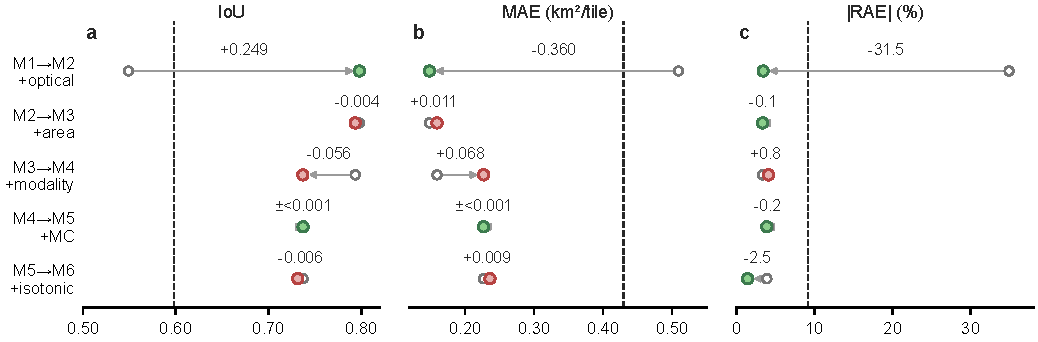
\includegraphics[width=0.90\textwidth,keepaspectratio]{../figures/fig_q2_ablation.pdf}
  \caption{Contribution of each component, M1 to M6}
  \label{fig:q2_ablation}
\end{figure}

Optical fusion is the decisive step: M1 to M2 raises IoU by 0.25 and cuts MAE$_A$ by 71\%. SAR-only M1 reaches IoU 0.549 and RAE $+34.9\%$, the measured cost of dropping the pre-flood land state, which alone separates a dark field or a permanent pond from new inundation; LightGBM paid no such cost because its features already contained NDWI. The area term changes little in-domain, modality dropout (a quarter of the training samples blinded) costs 0.06 IoU, and the MC mean leaves the metrics unchanged. Calibration cuts the total bias from $+4.1\%$ (M4) to $+1.45\%$: the tree stratum, $+74.87$\,km$^2$ of net error under LightGBM, contributes $-5.43$\,km$^2$ under M6, and the largest remaining nets are $+15.88$\,km$^2$ in wetland and $+15.20$\,km$^2$ in permanent water (Fig.~\ref{fig:q1_error_drivers}a).

Model choice was fixed before the test metrics were read: M2+MMU sets the in-domain ceiling at IoU 0.797, and M6 carries the SAR-only transfer because it pairs the calibrated area with a per-tile conformal interval, which is what Problem~3 consumes; its intervals cover the true tile area in 87.8\% of test tiles (folds 82.7--92.6\%, flood-share terciles 85.3--92.8\%) at a mean width of 0.54\,km$^2$.

\subsection{Data-Based Four-Level Intensity Grading}

Grading rests on the newly inundated area and its share of the study region, with explicit area or proportion thresholds. Because $\rho=A_{new}/A_{reg}$ is free of scale, thresholds are set on it and then translated into area thresholds for any unit:
\begin{equation}
A^*_g(A_{reg})=\theta_g\,A_{reg},\qquad g=1,2,3,
\label{eq:area_thr}
\end{equation}
with grade general for $\rho<\theta_1$, relatively strong for $\theta_1\le\rho<\theta_2$, strong for $\theta_2\le\rho<\theta_3$ and extremely strong for $\rho\ge\theta_3$. Round numbers are the wrong source for these cuts. The flood share of the 985 non-empty official tiles is strongly skewed; the fit is made on $x_t=\operatorname{logit}\rho^{ref}_t$ (with $\rho$ clipped to $[10^{-4},1-10^{-4}]$), a four-component Gaussian mixture by EM with 20 initializations. Adjacent components meet at their Bayes boundary, the root in $(\mu_g,\mu_{g+1})$ of
\begin{equation}
\pi_g\,\phi(x;\mu_g,s_g^2)=\pi_{g+1}\,\phi(x;\mu_{g+1},s_{g+1}^2),\qquad \theta_g=\frac{1}{1+e^{-x^*_g}},
\label{eq:gmm_bayes}
\end{equation}
where $\pi_g$, $\mu_g$, $s_g$ are the mixture weight, mean and standard deviation of component $g$ and $\phi$ the normal density. A tile sitting on the boundary is equally likely under both components, and the rule assigns it to the regime that most probably produced it. Fitted logit means are $-4.30$, $-1.85$, $1.24$ and $5.43$ with weights 0.544, 0.301, 0.098 and 0.057, which gives
\begin{equation}
\theta=(\theta_1,\theta_2,\theta_3)=(0.0593,\ 0.530,\ 0.969).
\label{eq:theta_values}
\end{equation}
Table~\ref{tab:grade_thr} translates them by \eqref{eq:area_thr} for three unit sizes.

\begin{table}[!ht]
\centering
\caption{Proportion and area thresholds of the four grades}
\label{tab:grade_thr}
\begin{tabular}{lcccc}
\toprule
Grade & $\rho$ range & Official tile 4.92\,km$^2$ & 1\,km$^2$ cell & Hengzhou 3440.4\,km$^2$ \\
\midrule
General & $<5.9\%$ & $<0.29$ & $<0.059$ & $<203.9$ \\
Relatively strong & 5.9--53.0\% & 0.29--2.61 & 0.059--0.530 & 203.9--1822.5 \\
Strong & 53.0--96.9\% & 2.61--4.77 & 0.530--0.969 & 1822.5--3333.5 \\
Extremely strong & $\ge96.9\%$ & $\ge4.77$ & $\ge0.969$ & $\ge3333.5$ \\
\bottomrule
\end{tabular}
\end{table}

How stable are these thresholds? We refit \eqref{eq:gmm_bayes} on 1000 block-bootstrap resamples of the 67 blocks. The 90\% intervals are $[0.0075,0.079]$ for $\theta_1$, $[0.067,0.655]$ for $\theta_2$ and $[0.522,0.998]$ for $\theta_3$, and 71\% of the resamples give a valid ordered four-component solution. The middle threshold is the least determined. BIC is lowest for two components (4604.8 against 4629.5 for four); the data alone do not demand four modes. Four grades are required by the problem, and the mixture is the most data-faithful way to place them. Jenks natural breaks on $x_t$ give $(0.035,0.371,0.967)$, close to the mixture for $\theta_1$ and $\theta_3$. The reference grades of the 1000 tiles are 575 general, 283 relatively strong, 89 strong and 53 extremely strong.

\subsection{How Area Errors Move the Grades}

A grade computed from an estimated area inherits its error. For unit $j$ we draw $m=1,\dots,M$ with $M=2000$ a residual $r^{(m)}$ from the pool $\mathcal R$ and a threshold vector $\theta^{(m)}$ from the bootstrap set:
\begin{equation}
\begin{split}
A_j^{(m)}&=\mathrm{clip}\big(\hat A_j+r^{(m)}\sigma'_j,\ 0,\ A_{reg,j}\big),\\
\pi_{jg}&=\frac1M\sum_{m=1}^M\mathbb 1\Big[G\big(A^{(m)}_j/A_{reg,j};\theta^{(m)}\big)=g\Big],\qquad
\sum_g\pi_{jg}=1,
\end{split}
\label{eq:grade_mc}
\end{equation}
where $G(\rho;\theta)$ is the grade of \eqref{eq:area_thr}. The vector $\pi_j$ replaces a single grade by a distribution that includes both the area error and the threshold uncertainty. Fig.~\ref{fig:q2_grading} shows the mixture fit and the resulting grade confusion.

\begin{figure}[t]
  \centering
  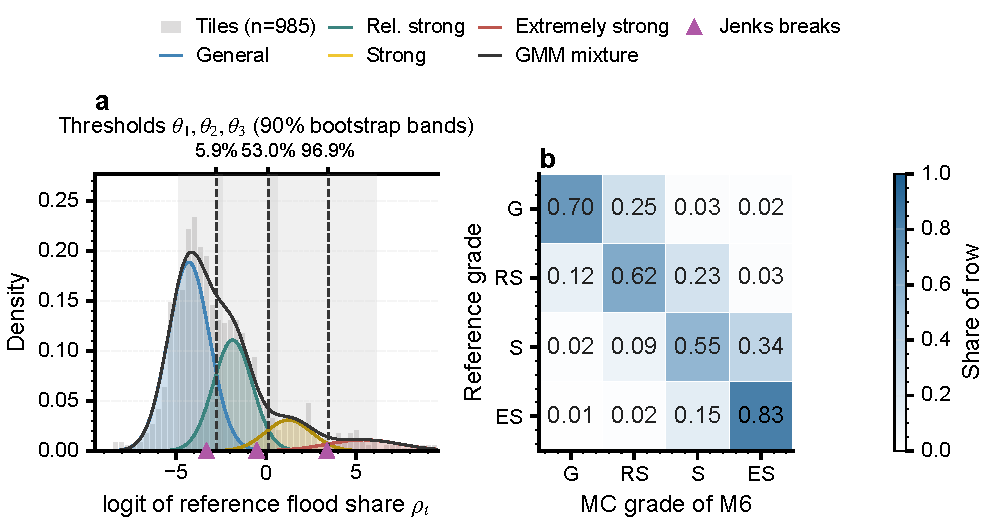
\includegraphics[width=0.90\textwidth,keepaspectratio]{../figures/fig_q2_grading.pdf}
  \caption{Gaussian-mixture grading and MC confusion}
  \label{fig:q2_grading}
\end{figure}

Where the two weakest regimes meet on the logit axis, the bootstrap bands of $\theta_1$ and $\theta_3$ stay narrow while that of $\theta_2$ widens (panel A). Row-normalized confusion against the Monte Carlo grade of M6 (panel B) keeps 70\% of the general, 62\% of the relatively strong, 55\% of the strong and 83\% of the extremely strong tiles in their grade, and the errors fall almost entirely into the neighboring grade. With the deterministic M6 area the grade is correct for 86.2\% of the tiles, against 54.3\% for LightGBM, so area calibration pays off directly in the grading. The expected Monte Carlo accuracy is 67.0\%, which prices in threshold uncertainty. Within four standardized errors of a threshold the flip probability $1-\max_g\pi_{jg}$ is 0.33--0.37, and 0.22 farther away; a unit near a threshold should therefore carry $\pi_j$ with its grade\cite{deepseek2026,qwen2026,doubao2026}.

Under a normal approximation of the signed tile-area error, Fig.~\ref{fig:q2_flip} makes the geometry explicit. Deep inside a grade the change probability is near zero; it peaks at one half exactly on a threshold, and the ridge widens with $\sigma$. Placing the 1000 test tiles in four bins at their mean estimated proportion and the standard deviation of their signed error gives $(1.1\%,0.026)$, $(10.2\%,0.098)$, $(32.1\%,0.141)$ and $(86.8\%,0.294)$. Two of the bins, the 5--20\% one and the highest, sit in the high-probability band of the surface -- consistent with the Monte Carlo flip rate of 0.33--0.37, even though most tiles lie far from $\theta_2$ and $\theta_3$.

\begin{figure}[!ht]
  \centering
  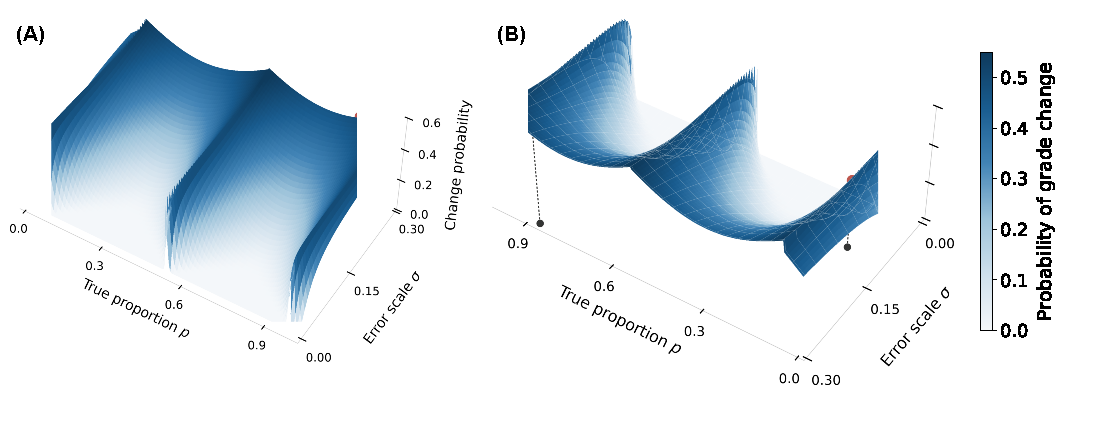
\includegraphics[width=0.90\textwidth,keepaspectratio]{../figures/fig_q2_flip_surface.pdf}
  \caption{Grade-change probability surface}
  \label{fig:q2_flip}
\end{figure}

\section[Problem 3]{Problem 3: Newly Inundated Area of Hengzhou with Guarded Model Transfer}
\label{sec:q3}

\subsection{Study Area and Choice of Imagery}

Hengzhou City lies on the Yu River in southern Guangxi. The study area is its GADM~4.1 boundary, $A_{reg}=3440.09$\,km$^2$ (nominal 3440.4\,km$^2$), as the problem asks for the proportion of the whole region; a second, physical denominator is the floodplain zone $\{\mathrm{REM}\le h^*\}$ inside the boundary, 2079.5\,km$^2$.

Rainy-season cloud rules out optics during the event, leaving radar as the observer. Sentinel-1 passes over Hengzhou exist on 27 June, 4 July and 16 July 2026; none falls on 6 July, so 27 June is the pre-flood baseline and 4 July (two days before the reference date) and 16 July (ten days after) serve as flood-time observations (Assumption~3). Products are terrain-corrected VV/VH backscatter in dB on a 10\,m grid at about 20\,m effective resolution; the latest cloud-free optical scene is Sentinel-2 of 31 May 2026.

\subsection{Verification of the Self-Collected Imagery}
\label{sec:q3_verify}

Before any model is applied, the Hengzhou layers have to be geometrically consistent with each other. We test this against a permanent-water reference $\mathcal W^{ref}=\{\mathrm{WC}=80\}\cap\mathrm{OSM}_{water}$, the pixels that both WorldCover and OSM map as water. Two independent sources agree there, so true water must appear dark in SAR. For each date we search the integer shift that maximizes the dark share on this reference,
\begin{equation}
(\Delta r,\Delta c)=\arg\max_{(\Delta r,\Delta c)}\ \frac{1}{|\mathcal W^{ref}|}\sum_{(r,c)\in\mathcal W^{ref}}\mathbb 1\big[VV(r+\Delta r,c+\Delta c)<-15\ \mathrm{dB}\big],
\label{eq:coreg}
\end{equation}
and correct the raster as $VV^{corr}(r,c)=VV(r+\Delta r,c+\Delta c)$.

At the delivered geotransform only 3.4\%, 4.4\% and 4.9\% of the reference water is SAR-dark on the three dates, which open water cannot be. Shifts of 5.4--6.2\,km north--south raise the dark share to 34.6\%, 35.6\% and 37.8\%. The three dates are also displaced against each other by up to 0.8\,km, without which the change guard would compare different ground. Problems 3, 4 and 5 all use the co-registered SAR. The optical scene fails the same test, 2.6\% of the reference water with $\mathrm{NDWI}>0$ at zero shift, at most 4.1\% under any translation, 35\% valid pixels; optics are absent everywhere in Hengzhou ($m_p=0$), the case M6 modality dropout was trained for, and the optical term drops out of $W_0$.

\subsection{Pre-flood Water and the Physics Detector}

A physics water detector $D_d$ on date $d$ uses the split-based Otsu rule \eqref{eq:ashman} on Lee-filtered VV in dB. On calibrated Sentinel-1 the literal rule with 64-pixel sub-blocks accepted land-cover contrasts as bimodal and labeled 52\% of the city as water at $-6.9$\,dB, the same failure as baseline A on the official tiles. We therefore use 128-pixel sub-blocks and accept a sub-block only if its dark class has a mean of at most $-15$\,dB, a physical condition for open water. The pooled thresholds are $-12.23$, $-12.02$ and $-12.80$\,dB for the three dates, from 245, 245 and 272 accepted sub-blocks. Pre-flood water is the union of independent sources (Assumption~4),
\begin{equation}
W_0=D_{0627}\ \cup\ \{\mathrm{WC}=80\}\ \cup\ \mathrm{OSM}_{water},
\label{eq:W0}
\end{equation}
with an area of 292.57\,km$^2$, of which 182.8\,km$^2$ come from the pre-flood SAR.

\subsection{Transfer of the Problem 2 Model}

Model weights do not change: the five fold models M6 of Problem~2 form an ensemble, each with two MC-dropout passes, ten passes per pixel. Checkpoint hashes equal those of Problem~2. What is mapped is the input representation, with the per-tile rank normalization of \eqref{eq:rank_norm} and the Lee filter of \eqref{eq:lee} on $256\times256$ tiles at 10\,m. Whether dB or linear amplitude $10^{VV/20}$ better resembles the GF-3 training input (Assumption~2) is settled by the two-sample Kolmogorov--Smirnov distance between the normalized Hengzhou land pixels and the official non-flood, non-water pixels,
\begin{equation}
T^\star=\arg\min_{T\in\{\mathrm{dB},\,\mathrm{amp}\}}\ \sup_x\Big|\hat F^{HZ}_{T}(x)-\hat F^{off}(x)\Big|,
\label{eq:ks}
\end{equation}
which is 0.106 for dB and 0.241 for amplitude, and dB is used. Refitting the isotonic map and the area-preserving threshold by \eqref{eq:isotonic}--\eqref{eq:tauA} on the pooled calibration predictions of the five members gives $\tau_A=0.557$.

\subsection{Physical Guards and the Final Sets}

A transferred model sees a new sensor, a new polarization (VV instead of HH) and no optics; its raw mask needs physical filtering. Three guards encode what flood water must satisfy. Water cannot stand far above the drainage network, which we measure by the relative elevation above the nearest mapped drainage, a Euclidean variant of the height above nearest drainage~\cite{nobre2011hand}:
\begin{equation}
\mathrm{REM}_p=\max\big(0,\ z^{DEM}_p-z^{DEM}_{n(p)}\big),\qquad n(p)=\arg\min_{q\in\mathcal D}\lVert \boldsymbol x_p-\boldsymbol x_q\rVert,
\label{eq:rem}
\end{equation}
where $\mathcal D$ is the drainage raster (OSM waterways and water polygons plus WorldCover water) and $z^{DEM}$ the Copernicus 30\,m elevation. New water must darken against the pre-flood pass by a margin $\delta$, as in change-detection chains~\cite{twele2016sentinel1}, and patches smaller than a minimum mapping unit of 50 pixels (0.5\,ha, about 12 independent looks at 20\,m resolution) are speckle. The newly inundated set on date $d$ is
\begin{equation}
\begin{split}
F_d=\mathrm{MMU}_{50}\Big(&\{\bar p\ge\tau_A\}\cap\overline{W_0}\cap\{\mathrm{REM}\le h^*\}\\
&\cap\{VV_d-VV_{0627}\le-\delta\}\Big),\qquad h^*=15\ \mathrm{m},\quad \delta=3\ \mathrm{dB},
\end{split}
\label{eq:F_hz}
\end{equation}
receded and flood-time water are
\begin{equation}
R_d=\big(W_0\cap D_{0627}\big)\setminus D_d,\qquad W_{1,d}=F_d\cup\big(W_0\setminus R_d\big).
\label{eq:W1_R}
\end{equation}
By construction $F_d\cap W_0=\emptyset$ and $F_d\subseteq W_{1,d}$. Both were confirmed on the saved rasters with zero violating pixels. A pre-flood water pixel counts as receded only if SAR saw it as water on 27 June and no longer sees it on date $d$. The literal alternative $W_{1,d}=F_d\cup(W_0\cap D_d)$ would also declare receded every mapped channel that SAR never resolves at 20\,m. It raises the receded area on 16 July from 79.44 to 180.09\,km$^2$ and is reported only for comparison. The areas follow \eqref{eq:def_F} and \eqref{eq:net_identity}:
\begin{equation}
A_{new,d}=\sum_{p\in F_d}a_p,\qquad A_{net,d}=A_{new,d}-\sum_{p\in R_d}a_p,\qquad \rho_d=\frac{A_{new,d}}{A_{reg}} .
\label{eq:areas_hz}
\end{equation}

\subsection{Newly Inundated Area, Net Increase and Proportion}

Table~\ref{tab:q3_results} gives the numbers the five questions require.

\begin{table}[!ht]
\centering
\caption{Newly inundated area by pass}
\label{tab:q3_results}
\begin{tabular}{lccccc}
\toprule
Date & $A_{new}$ (km$^2$) & $A_{net}$ (km$^2$) & $\rho$ & Grade & $\pi$ (G / RS / S / ES) \\
\midrule
4 July 2026 & 24.53 & $-54.70$ & 0.713\% & general & 0.74 / 0.25 / 0.010 / 0 \\
16 July 2026 & 26.90 & $-52.53$ & 0.782\% & general & 0.72 / 0.26 / 0.016 / 0 \\
\bottomrule
\end{tabular}
\end{table}

The newly inundated area is 24.53\,km$^2$ on 4 July and 26.90\,km$^2$ on 16 July, i.e. 0.71\% and 0.78\% of the city. All of it lies in the floodplain zone, where the proportion is 1.29\% on 16 July. By the thresholds of Table~\ref{tab:grade_thr} the city-level flood is ``general'' on both dates, with probability 0.72 on 16 July; the relatively-strong probability of 0.26 comes from bootstrap draws of $\theta_1$, whose lower 90\% bound of 0.75\% lies just below $\rho$. On 16 July the new flood covers 13.60\,km$^2$ of former cropland, 9.45\,km$^2$ of tree cover, 1.88\,km$^2$ of built-up land, 1.53\,km$^2$ of grassland and 0.43\,km$^2$ of bare land. The spatial distribution is shown in Fig.~\ref{fig:q3_newflood_map}.

The 27 June pass is the reference: $W_0$ is defined on it and $F$ is empty by construction, which leaves the two rows of Table~\ref{tab:q3_results} as the only comparable observations. Neither row observes the peak. 4 July precedes it, 16 July follows it by ten days, and that gap is exactly the interval in which the flood rose and fell. $A_{new}$ is a lower bound on the peak inundation; what the pair brackets is the receding limb and the residual water, the peak itself falling between the passes.

\begin{figure}[!ht]
  \centering
  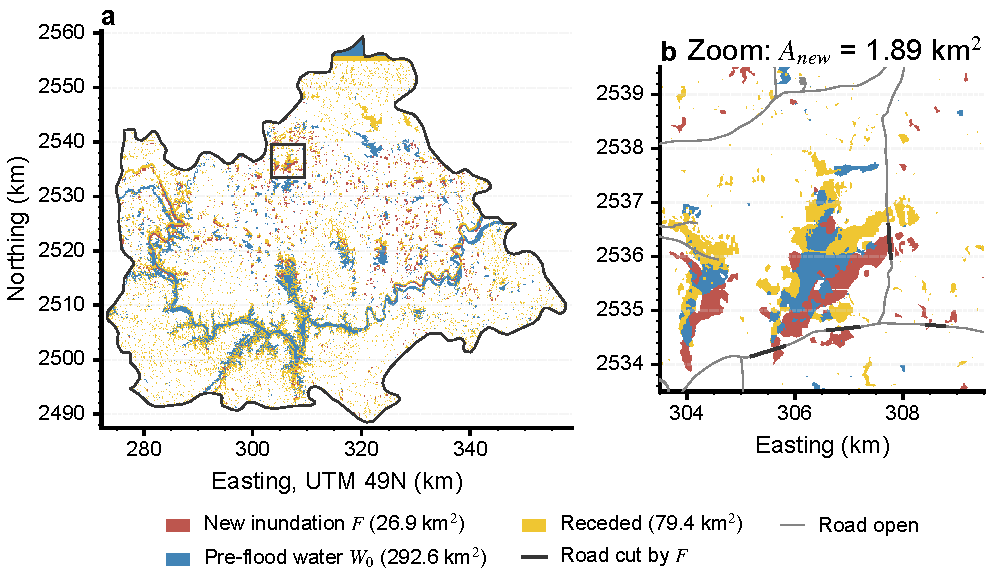
\includegraphics[width=0.90\textwidth,keepaspectratio]{../figures/fig_q3_newflood_map.pdf}
  \caption{Newly inundated area on 16 July 2026}
  \label{fig:q3_newflood_map}
\end{figure}

On 100\,m cells (panel A of Fig.~\ref{fig:q3_newflood_map}) the new inundation follows the Yu River and its tributaries as narrow bands along the valley floors, and the receded water lies on the same corridors. The $6\times6$\,km window with the largest new area is shown at the full 10\,m resolution in panel (B), where flooded fields touch the road network. Those road cuts feed Problem~5. One artifact needs a word: the horizontal band near northing 2555\,km, an edge left by the 27 June co-registration shift where pre-flood SAR is invalid, inflates $W_0$ and $R$ by about 3.4\,km$^2$ each. It carries no new inundation; $A_{new}$, $\rho$ and everything downstream are unaffected, while $A_{net}$ is about 3.4\,km$^2$ too negative.

\begin{figure}[!ht]
  \centering
  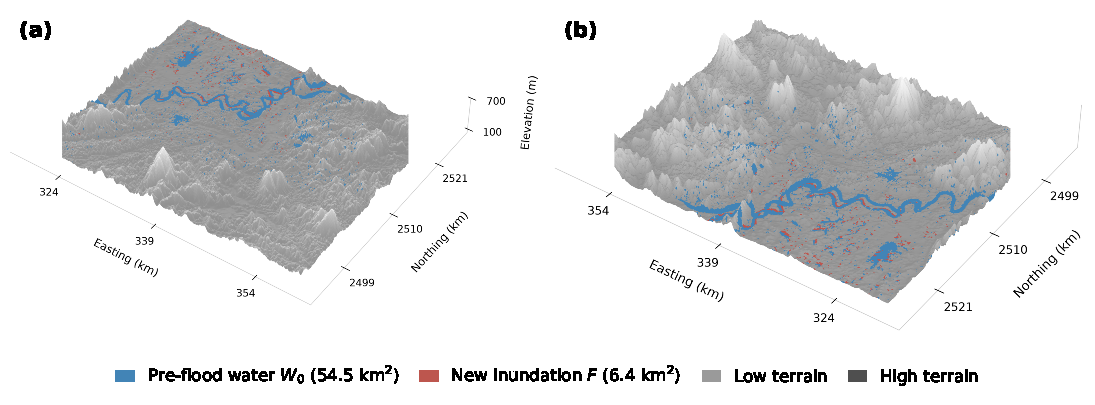
\includegraphics[width=0.90\textwidth,keepaspectratio]{../figures/fig_q3_terrain.pdf}
  \caption{New inundation on the DEM}
  \label{fig:q3_terrain}
\end{figure}

Fig.~\ref{fig:q3_terrain} places those masks on the terrain. The 40$\times$32\,km window is the one with the densest new inundation. It contains 6.4\,km$^2$ of $F$ and 54.5\,km$^2$ of $W_0$, about a quarter and a fifth of the city totals. Every new pixel lies below 200\,m (median 58\,m) and follows the valley floor, whereas the eastern ridge rises to 710\,m and stays dry: the flood is a corridor phenomenon, not a sheet.

Table~\ref{tab:q3_budget} answers why the net increase is negative while new inundation is positive.

\begin{table}[!ht]
\centering
\caption{Guard cascade and water balance (km$^2$)}
\label{tab:q3_budget}
\small
\setlength{\tabcolsep}{3pt}
\renewcommand{\arraystretch}{0.92}
\begin{tabular*}{\textwidth}{@{}l@{\extracolsep{\fill}}rrrr@{\hspace{14pt}}lrr@{}}
\toprule
\multicolumn{5}{c}{Guard cascade} & \multicolumn{3}{c}{Water balance} \\
\cmidrule(lr){1-5}\cmidrule(lr){6-8}
Stage & \multicolumn{2}{c}{4 July} & \multicolumn{2}{c}{16 July} & Term & & \\
\cmidrule(lr){2-3}\cmidrule(lr){4-5}
 & Remaining & Removed & Remaining & Removed & & 4 July & 16 July \\
\midrule
Raw model              & 146.52 & --    & 154.43 & --    & $W_0$             & 292.57 & 292.57 \\
After $W_0$ guard      &  68.43 & 78.09 &  68.85 & 85.58 & Receded $R$       &  79.23 &  79.44 \\
After REM guard        &  44.95 & 23.48 &  44.74 & 24.11 & New $A_{new}$     &  24.53 &  26.90 \\
After $\Delta$VV guard &  34.32 & 10.63 &  36.98 &  7.76 & $W_1$             & 237.87 & 240.03 \\
After MMU              &  24.53 &  9.79 &  26.90 & 10.08 & Net $A_{net}$     & $-54.70$ & $-52.53$ \\
\bottomrule
\end{tabular*}
\end{table}

The balance explains the negative net increase: SAR sees 79.4\,km$^2$ on 27 June that is gone by 16 July, three times the new inundation, 72.4\,km$^2$ of it outside every mapped source (49.4 under tree cover, 16.7 under cropland) and 7.04\,km$^2$ in permanent channels and reservoirs. New water of 26.90 against 79.44 of recession gives $A_{net}=-52.54$ by \eqref{eq:net_identity}, a water-balance quantity rather than the size of the flood; the two flood-time passes agree on the recession to 0.3\% (the literal $-153.19$ comes from the wider 4 July recession). Narrowing the baseline would move the sign: with static water bodies alone (143.4\,km$^2$), the 61.1\,km$^2$ still standing on 16 July would enter $F$ and raise $A_{new}$ from 26.90 to about 88\,km$^2$.

The cascade of \eqref{eq:F_hz} steps from 154.43\,km$^2$ raw to 26.90\,km$^2$ final on 16 July, removing 82.6\% (83.3\% on 4 July), mostly permanent water scored at 0.285 mean probability and excluded by $W_0$. What holds the Hengzhou estimate is the physics guards---drainage, terrain, multi-date change---evidence independent of the network.

\subsection{Transfer Checks and Sensitivity}

Without labels, credibility comes from consistency. The unguarded model mask and the physics change mask $\{\Delta VV\le-3\}\cap D_d\setminus W_0$ overlap at IoU 0.207 with area ratio 2.60: the model sees more candidate water than radar change alone. The VV histogram is bimodal on 16 July (Ashman $D=3.53$) and weakly on 4 July ($D=1.92$); the two new-inundation sets agree at Jaccard 0.391, partial across ten days. The $W_0$ variants order correctly: the union contains the SAR-only $W_0$, so removing it can only shrink $F$, and $A_{new}$ with SAR-only is larger (30.47\,km$^2$). Closing $W_0^{\mathrm{union}}\supseteq W_0^{\mathrm{sar+wc}}\supseteq W_0^{\mathrm{sar}}$ at $26.90<27.29<30.47$\,km$^2$, the 1.4\% step coming from dropped OSM vectors; grade, zone ranking (Spearman 0.996) and the six open depots are identical for both permanent-water variants.

Neither guard parameter $h^*$ nor $\delta$ nor the probability threshold has Hengzhou data to fix it. Fig.~\ref{fig:q3_threshold_surface} recomputes $A_{new}$ over 30 combinations of a threshold shift $\Delta\tau\in\{-0.2,\dots,0.2\}$ and $h^*\in\{5,10,15,20,30,\infty\}$\,m, plus one-at-a-time changes of the other settings.

\begin{figure}[!ht]
  \centering
  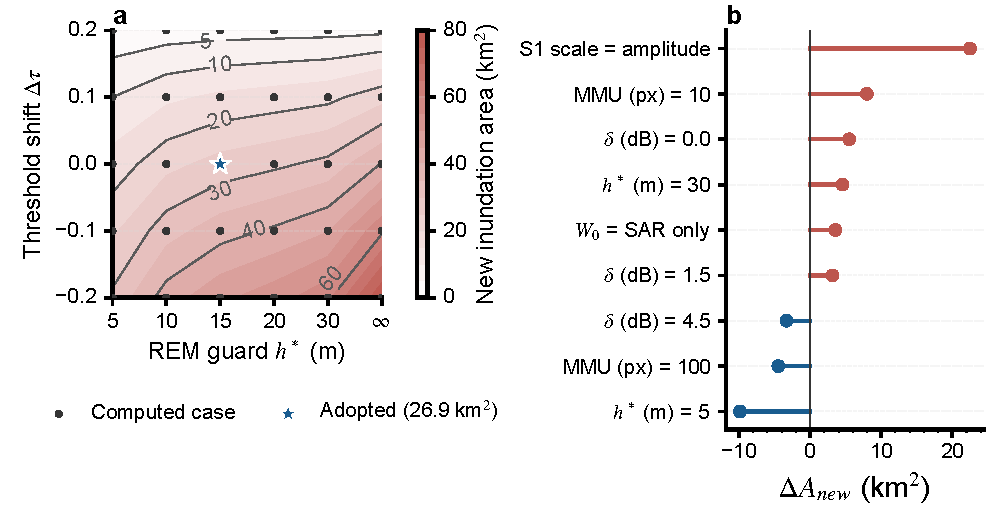
\includegraphics[width=0.90\textwidth,keepaspectratio]{../figures/fig_q3_threshold_surface.pdf}
  \caption{Sensitivity of the Hengzhou new area}
  \label{fig:q3_threshold_surface}
\end{figure}

Panel (A) rises with $h^*$ and falls with $\Delta\tau$, as the guards require: over the grid $A_{new}$ spans 1.57 to 79.52\,km$^2$, and that band travels into every downstream answer. Change margin, water definition, amplitude scale and MMU vary comparably in panel (B) (Table~\ref{tab:sens_chain}). The grade stays ``general'' everywhere, the largest $\rho$ 2.3\% against $\theta_1=5.9\%$: area responds to the guards, the grade does not.

Treating the tile errors of \eqref{eq:conformal} as independent, as in Problem~2, gives $[13.48,40.33]$\,km$^2$ on 16 July, a band that contains the scenario values of the main settings\cite{deepseek2026,qwen2026,doubao2026}.

A target-domain intercept can be priced against physics: new water is dark, low and outside $W_0$ ($\Delta VV\le-6$\,dB, $\mathrm{REM}\le5$\,m, $W_0$ false, 527\,790 pixels), upland bright and high ($\mathrm{REM}\ge30$\,m, $\Delta VV\ge+2$\,dB, 1\,855\,718). The transferred field averages 0.245 and 0.040 on the two anchors, conservative where the physics is certain. Restoring the 22\% prevalence needs $b=+1.19$, which alone moves the raw mask from 154.45 to 415.89\,km$^2$ (2.7$\times$): $\tau_A$ already acts as an intercept, lowering the field so the mask matches the source calibration, and a second intercept read off physics undoes that correction. The two cannot be stacked; we keep $\tau_A$, verifiable on labels, and record $b=+1.19$ as the residual. With 0.285 assigned to permanent water, the flood is recovered from the guards, not from a field deliberately low after two transfers.

\section[Problem 4]{Problem 4: Hazard--Exposure--Response Assessment on Settlement Catchments}
\label{sec:q4}

\subsection{Assessment Units}

Township boundaries of Hengzhou are not publicly available, and the 17 towns are too few for objective weighting or for a meaningful relief model. We take as units the Voronoi cells of all 393 OSM settlement nodes (370 villages, 16 towns, 5 hamlets, one city node and one suburb), clipped to the city boundary. A cell is the area that is closer to its settlement than to any other, i.e. the natural catchment that relief for that settlement would serve. The cells partition the boundary exactly (sum 3440.0919\,km$^2$ against 3440.0920\,km$^2$), and the new inundation of the units sums to the city value of Problem~3 (26.9025\,km$^2$, relative difference $4\times10^{-9}$). Each unit inherits the town or city zone of its nearest town or city node, which gives 17 zones for reporting. A unit counts as affected if $A_{new,j}$ is at least one minimum mapping unit, 0.005\,km$^2$. 259 of the 393 units are affected, and only these are scored.

\subsection{Indicator System}

The core indicators are newly inundated area, proportion and intensity; exposure of people and critical facilities enters as the fourth. Every indicator in Table~\ref{tab:q4_ind} is an overlay of the Problem~3 raster $F_{0716}$ with a public layer; the assessment changes whenever $F$ changes. All indicators are oriented so that larger means worse.

\begin{table}[!ht]
\centering
\caption{Indicators of the regional assessment}
\label{tab:q4_ind}
\small
\begin{tabular}{p{0.13\textwidth}p{0.28\textwidth}p{0.35\textwidth}p{0.11\textwidth}}
\toprule
Criterion & Indicator & Definition & Weight \\
\midrule
Hazard & H1 new area $A_{new,j}$ (km$^2$) & $\sum_{p\in F\cap j}a_p$ & 0.233 \\
 & H2 proportion $\rho_j$ & $A_{new,j}/A_{reg,j}$ & 0.198 \\
 & H3 intensity $I_j$ & expected grade $\sum_g g\,\pi_{jg}$ by \eqref{eq:grade_mc} & 0.108 \\
Exposure & E1 flooded population & $\sum_c \mathrm{pop}_c\,\phi_c$, $\phi_c$ flooded share of 100\,m cell $c$ & 0.055 \\
 & E2 flooded built-up (km$^2$) & $|F\cap\{\mathrm{WC}=50\}|_a$ & 0.055 \\
 & E3 flooded cropland (km$^2$) & $|F\cap\{\mathrm{WC}=40\}|_a$ & 0.047 \\
 & E4 exposed facilities & facility proxies within 500\,m of $F$ & 0.140 \\
Response & R1 access time (min) & flood-cut network time from the flooded-population centroid to the nearest unflooded facility proxy & 0.080 \\
 & R2 road-cut share & impassable road length / road length in the unit & 0.084 \\
\bottomrule
\end{tabular}
\end{table}

Terrain enters through the REM guard inside $F$. Built-up land is taken from WorldCover because OSM holds only 609 building footprints. Hospitals and shelters are represented by the facility proxies of Assumption~5 (town and city nodes plus schools), because OSM lists only five service points. A road edge is impassable if any of its sample points, taken every 20\,m, lies within 20\,m of $F$. Unreachable units get twice the largest finite access time, 165.6\,min. Over the whole city the overlay finds 13,954 flooded people, 1.88\,km$^2$ of flooded built-up land, 13.60\,km$^2$ of flooded cropland, 8 of 22 facility proxies within 500\,m of new inundation, and 117.4 of 2542.3\,km of roads cut. 75 affected units have no road path to an unflooded facility.

At 1\,km the two fields separate rather than co-vary (Fig.~\ref{fig:q4_grid1km}). Across the 1010 cells that carry new inundation the rank correlation of water area with resident population is $\rho_S=0.36$; the ten cells with the largest area hold 8.2\% of the flooded population, and the ten that hold the most people carry 4.9\% of the new water. A cell can be nearly dry and still shelter several hundred people; exposure is not a rescaling of the flood map, and the exposure criterion carries its own population and facility indicators instead of weighting area alone. Panels (A) and (B) of Fig.~\ref{fig:q4_grid1km} map the two fields and panel (C) their joint distribution, with the ten largest areas and the ten most populated cells ringed.

\begin{figure}[!ht]
  \centering
  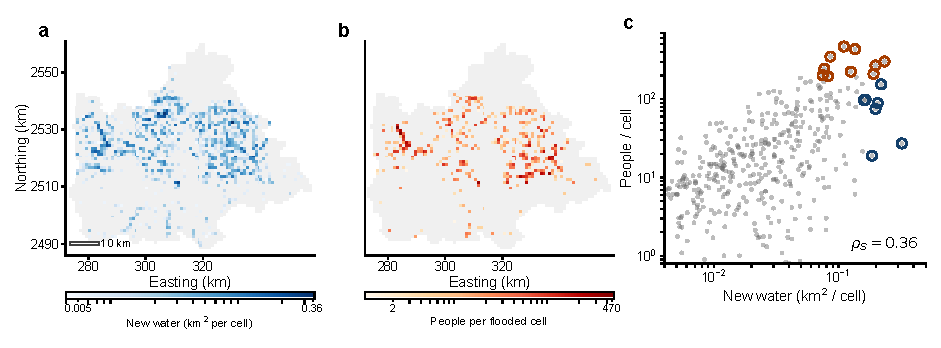
\includegraphics[width=0.90\textwidth,keepaspectratio]{../figures/fig_q4_grid1km.pdf}
  \caption{A 1\,km exposure layer over the mapped new inundation}
  \label{fig:q4_grid1km}
\end{figure}

\subsection{Combined Weights and the TOPSIS Index}

Indicators are min--max normalized over units, $r_{jk}=(X_{jk}-\min_jX_{jk})/(\max_jX_{jk}-\min_jX_{jk})$. Inside each criterion two objective weightings are combined. Entropy weights $w^e_k\propto1-e_k$ with $e_k=-\frac{1}{\ln n}\sum_j\tilde r_{jk}\ln\tilde r_{jk}$ and $\tilde r_{jk}=r_{jk}/\sum_jr_{jk}$ reward discrimination between units. CRITIC weights~\cite{diakoulaki1995critic} $w^c_k\propto s_k\sum_l(1-\mathrm{corr}_{kl})$ reward variation that is not redundant. The game-theoretic combination chooses the mix closest to both:
\begin{equation}
\begin{bmatrix}w^e\!\cdot\!w^e & w^e\!\cdot\!w^c\\ w^c\!\cdot\!w^e & w^c\!\cdot\!w^c\end{bmatrix}
\begin{bmatrix}\alpha_1\\ \alpha_2\end{bmatrix}=
\begin{bmatrix}w^e\!\cdot\!w^e\\ w^c\!\cdot\!w^c\end{bmatrix},\qquad
w^{(c)}=\frac{|\alpha_1|w^e+|\alpha_2|w^c}{|\alpha_1|+|\alpha_2|}.
\label{eq:game_weights}
\end{equation}
For the hazard criterion, entropy gives (0.477, 0.404, 0.119) and CRITIC (0.320, 0.273, 0.407), and the combination with $\alpha=(0.767,0.303)$ gives (0.432, 0.367, 0.201). Between criteria we use a judgment that follows the problem text, hazard as core, exposure second, response third, through the AHP matrix
\begin{equation}
J=\begin{bmatrix}1&2&3\\ 1/2&1&2\\ 1/3&1/2&1\end{bmatrix},\qquad
\Omega=\text{principal eigenvector of }J,\qquad
\mathrm{CR}=\frac{(\lambda_{max}-3)/2}{0.58},
\label{eq:ahp}
\end{equation}
which gives $\Omega=(0.540,0.297,0.163)$ with $\lambda_{max}=3.0092$ and $\mathrm{CR}=0.0079<0.1$. The final weights $w_k=\Omega_{c(k)}w^{(c(k))}_k$ sum to one and are listed in Table~\ref{tab:q4_ind}. The three core hazard indicators carry 0.539 of the total weight. The disaster index is the TOPSIS closeness on $v_{jk}=w_kr_{jk}$,
\begin{equation}
S_j=\frac{D^-_j}{D^+_j+D^-_j},\qquad D^\pm_j=\big\lVert v_j-v^\pm\big\rVert_2,\qquad v^+_k=\max_jv_{jk},\ v^-_k=\min_jv_{jk},
\label{eq:topsis}
\end{equation}
so $S_j=1$ for a unit at the worst observed value of every indicator. Four disaster levels (I most severe) are formed by Jenks natural breaks of $S_j$. Zones are scored analogously from aggregated indicators.

\subsection{Spatial Pattern of Disaster Severity}

Levels hold 3 units in Level~I, 28 in Level~II, 96 in Level~III and 132 in Level~IV. Whether severity follows the flood alone, or exposure reorders it, is visible in Fig.~\ref{fig:q4_risk_map}, a bivariate map crossing hazard ($H_1$) with exposure ($E_1$), each split at the tertiles of the affected units.

\begin{figure}[!ht]
  \centering
  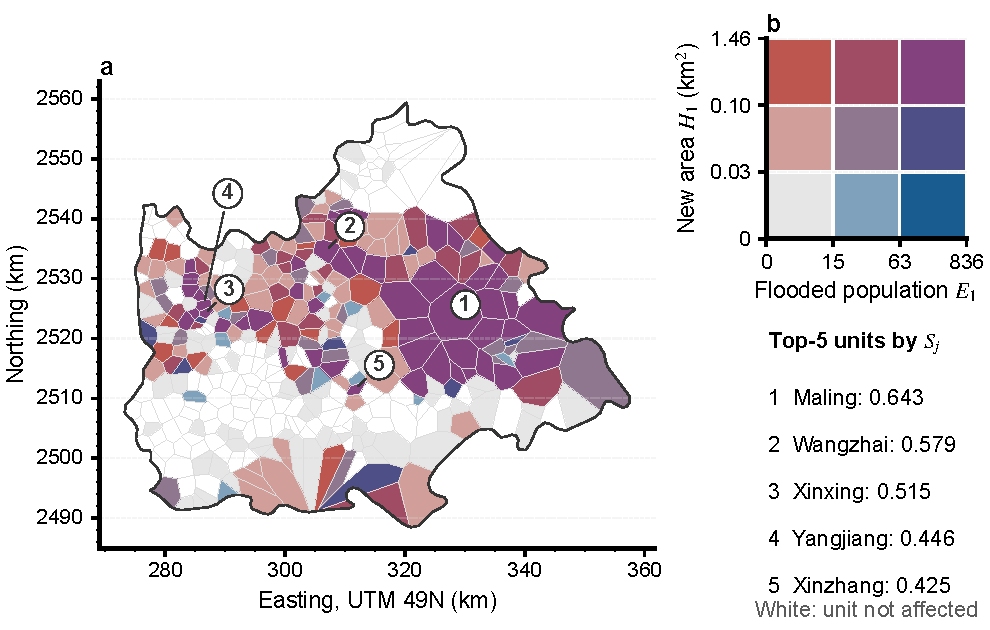
\includegraphics[width=0.90\textwidth,keepaspectratio]{../figures/fig_q4_risk_map.pdf}
  \caption{Hazard--exposure map of the 393 units}
  \label{fig:q4_risk_map}
\end{figure}

One belt carries the disaster: between northings 2520 and 2535\,km lie 16.78 of the 26.90\,km$^2$ of new inundation and 8298 of the 13,954 flooded people, with the Luancheng, Shitang, Maling and Yunbiao zones; south of northing 2505\,km, 56 units share 1.15\,km$^2$ and 237 people. Five catchments stand out: Maling town ($S=0.643$; 1.46\,km$^2$; 836 people; an exposed facility; no road access to an unflooded one), Wangzhai in the Shitang zone ($0.579$; 118 people; 9.2\% of its area newly wet), Xinxing ($0.515$) and Yangjiang ($0.446$) in Luancheng (13.2\% and 9.0\%), and Xinzhang in Liantang ($0.425$).

At zone level Shitang ranks first ($S=0.787$; 4.91\,km$^2$, 1189 people), then Maling (0.760; 2.96\,km$^2$, 2305 people), Luancheng (0.740; 3.58\,km$^2$, 2144 people), Yunbiao (0.648), Xiaoyi (0.558) and Nayang (0.501), all with flood shares of only 1.1--2.4\%. These are zone-level shares, not the city-level thresholds of Table~\ref{tab:grade_thr}: on a 243\,km$^2$ zone the same share means a tenth of the absolute area it does over the 3440\,km$^2$ city, and the four levels come from the Jenks breaks of $S_j$, not from the intensity table. Where the flood meets people and cut roads drives the ranking, not large flooded areas.

A stricter test grades on the other dimension: replacing the share $\rho_j$ with the absolute area $A_{new,j}$ -- a four-component Gaussian mixture on $\log_{10}A_{new,j}$ with boundaries 4.83, 9.32 and 21.39\,km$^2$ -- lifts 16 of the 259 affected units by one level, lowers none, and touches 433.4\,km$^2$ of the city. Spearman between the two gradings is 0.973; grading on area alone drops it to 0.749. What gets rewritten are the large-but-thin units a share-only rule understates, so the level assignment is stable to which dimension of the hazard is graded.

\subsection{Robustness of the Ranking}

A ranking used for relief must not depend on a particular weight vector. We draw $M=2000$ weight sets with $\Omega\sim\mathrm{Dir}(50\,\Omega_0)$ and $w^{(c)}\sim\mathrm{Dir}(50\,w^{(c)}_0)$ around the baseline, recompute the ranking each time, and compare it with rankings from hazard indicators only and from alternative Problem~3 inputs. Fig.~\ref{fig:q4_rank_robustness} summarizes the outcome.

\begin{figure}[!ht]
  \centering
  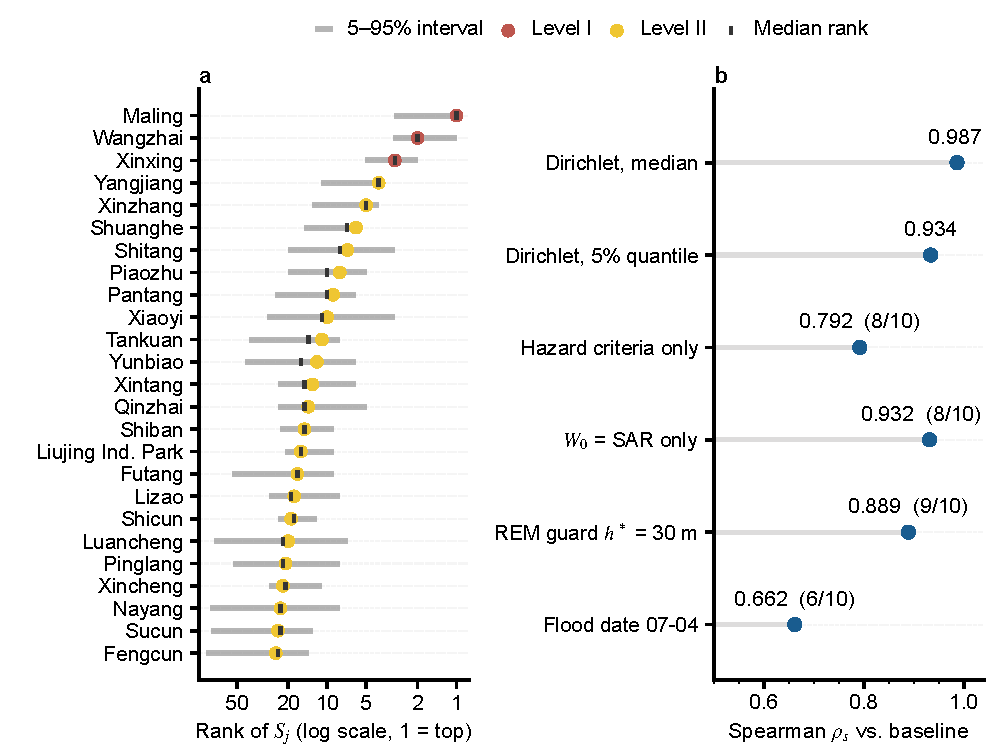
\includegraphics[width=0.90\textwidth,keepaspectratio]{../figures/fig_q4_rank_robustness.pdf}
  \caption{Robustness of the unit ranking}
  \label{fig:q4_rank_robustness}
\end{figure}

Weight perturbation leaves the ranking essentially unchanged: median Spearman against the baseline is 0.987, its 5\% quantile 0.934, and the 5--95\% rank intervals of the top units in panel (A) are narrow. Ranking by hazard alone gives 0.792 and keeps 8 of the top 10; exposure and response reorder about a fifth of the ranking, which is why they are there. Input data matter more than weights. With the 4 July flood the correlation falls to 0.662, while the SAR-only $W_0$ and the 30\,m guard leave it at 0.932 and 0.889 (Table~\ref{tab:sens_chain}). The ranking is a statement about the 16 July observation, and the letter turns that into a recommendation to recompute it after each pass\cite{deepseek2026,qwen2026,doubao2026}.

\section[Problem 5]{Problem 5: Depot Activation and Relief Allocation on the Flood-Cut Network}
\label{sec:q5}

\subsection{Task, Decision Time and Demand}

Among the tasks offered by the problem we choose emergency supply allocation combined with the choice of which relief depots to open: on a given day, which of the candidate depots should be activated, and how many tonnes of daily relief kits should each open depot send to each affected settlement catchment over the road network that is still passable. The main decision time is $T_0=16$ July 2026, the moment the Sentinel-1 pass of that day has been processed. As a second decision time we use 4 July, to measure what the later pass is worth.

Demand comes directly from Problem~4. With the flooded population $P_j$ of unit $j$ and the relief need of Assumption~6,
\begin{equation}
d_j=\frac{q\,H\,P_j}{1000}\ \ [\mathrm t],\qquad q=3.5\ \mathrm{kg\,person^{-1}\,day^{-1}},\quad H=3\ \mathrm d,
\label{eq:demand}
\end{equation}
and the priority of the unit is its disaster index, $w_j=\max(S_j,0.001)$. The floor keeps the lowest-ranked affected unit in the objective. Affected units with at least one flooded person form 164 demand units with a total demand of 146.46\,t.

\subsection{Flood-Cut Network and Admissible Assignments}

OSM roads are snapped at 1\,m into a directed graph (one-way tags respected) with edge time equal to length over a class speed reduced for emergency driving (80\,km/h on motorways down to 15\,km/h on tracks). Every edge that touches the 16 July raster $F$ under the 20\,m buffer rule is deleted. 117.4\,km of road disappear. The flooded-population centroid of each unit is connected to the nearest node of the cut graph by an access leg of at most 5\,km at 15\,km/h. Candidate depots are the 16 town nodes, the city node and the schools, merged within 300\,m to 21 candidates. A candidate is excluded if it lies within 100\,m of $F$ or more than 1\,km from the cut graph, which leaves 20. The travel time $t_{ij}$ is the depot access time plus the Dijkstra time on the cut graph plus the demand access time, infinite if no path exists, and the admissible pairs are
\begin{equation}
\mathcal A=\{(i,j):\ t_{ij}\le T_{max}\},\qquad T_{max}=120\ \mathrm{min}.
\label{eq:admissible}
\end{equation}
This gives 1189 admissible pairs. For 57 demand units no candidate is admissible: the flood has cut every road path to them within two hours. In this way the image result enters the optimization twice, through the deleted roads and depots and through $d_j$ and $w_j$.

\subsection{A Bi-objective Location--Allocation MILP}

\textbf{Decision variables.} Opening a depot is a yes-or-no decision, so the depot variable is binary:
\begin{equation}
\eta_i=\begin{cases}1, & \text{candidate depot } i \text{ is activated on the decision day},\\ 0, & \text{otherwise},\end{cases}\qquad i\in\mathcal I,\ |\mathcal I|=20 .
\label{eq:eta}
\end{equation}
The shipment $x_{ij}\ge0$ (tonnes from depot $i$ to unit $j$, defined only for $(i,j)\in\mathcal A$) and the unmet demand $u_j\ge0$ are continuous, because relief kits are counted in thousands and their tonnage is effectively divisible.

\textbf{Objectives.} Resources are limited, so relief has to serve ``areas and populations in urgent need of assistance in a more timely and targeted manner''. ``Targeted'' is measured by the priority-weighted unmet share and ``timely'' by the priority-weighted delivery time, both minimized:
\begin{equation}
\min\ f_1=\frac{\sum_jw_ju_j}{\sum_jw_jd_j},\qquad
\min\ f_2=\frac{\sum_{(i,j)\in\mathcal A}w_j\,t_{ij}\,x_{ij}}{\sum_jw_jd_j}\ \ [\mathrm{min}].
\label{eq:q5_obj}
\end{equation}
Both are normalized by the same weighted demand, so $f_1\in[0,1]$ and $f_2$ is an average delivery time in minutes per weighted tonne.

\textbf{Constraints.}
\begin{equation}
\begin{aligned}
\text{s.t.}\quad
&\sum_{i:(i,j)\in\mathcal A}x_{ij}+u_j=d_j, && \forall j,\\
&\sum_{j:(i,j)\in\mathcal A}x_{ij}\le C_i\,\eta_i, && \forall i\in\mathcal I,\\
&x_{ij}\le d_j\,\eta_i, && \forall (i,j)\in\mathcal A,\\
&\sum_{i\in\mathcal I}\eta_i\le K,\\
&\sum_{(i,j)\in\mathcal A}\frac{2t_{ij}+t_l}{Q_v}\,x_{ij}\le 60\,N_vT_sH,\\
&x_{ij}\ge0,\quad u_j\ge0,\quad \eta_i\in\{0,1\}.
\end{aligned}
\label{eq:q5_cons}
\end{equation}
Each unit's demand is balanced between deliveries and unmet need, and no shortfall can hide. Tonnage is capped at the depot's horizon capacity ($C_i=60$\,t for a town or school, 200\,t for the city) and, through $\eta_i$, only open depots may ship; this is the standard linear form of a fixed opening decision, $C_i$ being the tightest valid bound; no artificial constant is needed. The linking bound $x_{ij}\le d_j\,\eta_i$ is redundant for integer solutions and tightens the LP relaxation, since no unit can receive more than its demand from one depot. Staff and stock for more than $K=6$ sites are not available. What remains is the fleet budget: a round trip of $2t_{ij}$ plus $t_l=30$\,min for loading carries $Q_v=5$\,t, and $N_v=40$ trucks working $T_s=12$\,h per day over $H=3$ days provide $60N_vT_sH=86{,}400$ vehicle-minutes. Aggregate vehicle-minutes, not a routing model; the time limit enters through $\mathcal A$.

\textbf{Model class and solution method.} The model is a mixed-integer linear program with 20 free binary variables (the excluded candidate is fixed closed) and 1353 continuous variables (1189 shipments, 164 unmet demands), and 1375 structural constraints (164 balances, 20 capacities, 1189 linking bounds, one depot limit, one fleet budget). With only 20 binaries an exact branch-and-bound solve is cheap; no heuristic is needed. We use the HiGHS solver~\cite{huangfu2018highs} with relative gap 0. The recommended plan is lexicographic, because covering need is more important than speed: stage 1 computes $f_1^*=\min f_1$ subject to \eqref{eq:q5_cons}, stage 2 minimizes $f_2$ subject to \eqref{eq:q5_cons} and $f_1\le f_1^*+10^{-6}$. The trade-off is then traced by the $\varepsilon$-constraint method, $\min f_2$ subject to $f_1\le\varepsilon_k$ with $\varepsilon_k=f_1^*+\frac{k}{14}(1-f_1^*)$ for $k=0,\dots,14$, and the knee is the front point farthest from the chord between its end points on normalized axes. Every solve returned status optimal with zero gap.

\subsection{Recommended Relief Plan for 16 July}

The lexicographic solve opens six depots. Table~\ref{tab:q5_plan} lists them with their shipments.

\begin{table}[H]
\centering
\caption{Open depots of the recommended plan}
\label{tab:q5_plan}
{\small\renewcommand{\arraystretch}{0.86}
\begin{tabularx}{\dimexpr\linewidth-4.6pt\relax}{l*{3}{>{\centering\arraybackslash}X}}
\toprule
Depot & Type & Capacity (t) & Shipped (t) \\
\midrule
Taoxu & town & 60 & 39.59 \\
Yunbiao & town & 60 & 28.82 \\
Shitang & town & 60 & 5.65 \\
Gaocun & school & 60 & 1.97 \\
Zhenlong & town & 60 & 0.66 \\
Liujing & town & 60 & 0.13 \\
\midrule
Total & & 360 & 76.82 \\
\bottomrule
\end{tabularx}}
\end{table}

The plan reaches $f_1^*=0.570$ and $f_2=13.05$\,min. It ships 76.82 of the 146.46\,t demanded and serves 7316 of the 13,948 people in the demand units. Fig.~\ref{fig:q5_route_alloc} draws the delivery paths on the cut network.

\begin{figure}[H]
  \centering
  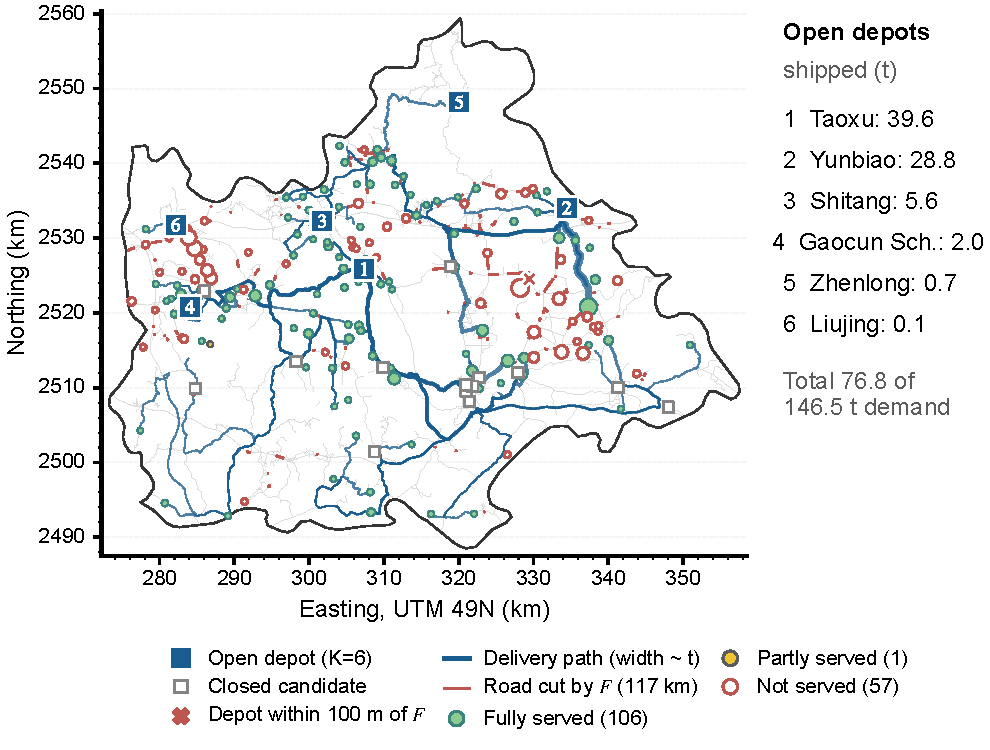
\includegraphics[width=0.98\textwidth,keepaspectratio]{../figures/fig_q5_route_alloc.pdf}
  \caption{Recommended relief plan}
  \label{fig:q5_route_alloc}
\end{figure}

Taoxu and Yunbiao, the two largest depots, supply 89\% of the tonnage through short paths into the central and eastern flood belt; Shitang and the Gaocun school serve the north and west; Zhenlong and Liujing cover small remote demands. More than half of the weighted demand stays unmet even though the open depots hold 360\,t, almost 2.5 times the total demand, and the fleet uses 1497 of 86,400 vehicle-minutes. Capacity is not the bottleneck, and neither are trucks. Reachability is. Water cuts off the 57 units that have no admissible depot, and no allocation over the road network can reach them. To six decimals the optimum equals the weighted demand of those 57 units (0.569927, against $f_1^*=0.569928$); the allocation carries no slack, every reachable unit is served in full, and no shipment on this network can lower $f_1$. Operationally this is the finding that matters, and it is why the letter asks for boats and helicopters for these units.

\begin{table}[H]
\centering
\caption{The flood map as an input to the relief plan}
\label{tab:q5_nomap}
{\small\renewcommand{\arraystretch}{0.86}
\begin{tabularx}{\dimexpr\linewidth-4.6pt\relax}{l*{3}{>{\centering\arraybackslash}X}}
\toprule
Plan & $f_1$ & $f_2$ (min) & Served \\
\midrule
MILP on 16 July (recommended) & 0.570 & 13.05 & 7316 \\
Same model, flood map withheld & 0.001 & 14.55 & 13924 \\
\quad replayed on the real cut network & 0.592 & 20.52 & 6997 \\
Greedy nearest-depot & 0.573 & 9.47 & 7237 \\
Proportional to depot capacity & 0.570 & 19.55 & 7316 \\
\bottomrule
\end{tabularx}}
\end{table}

Table~\ref{tab:q5_nomap} prices the flood map itself. Withheld from the model, the same objective reports a nearly perfect plan: $f_1=0.001$, 13,924 people served. Replayed on the network the water actually cut, that plan serves 6,997 people at $f_1=0.592$ -- 318 fewer than the plan that saw the map -- and takes 20.52\,min against 13.05. The map is not a refinement of the answer; it is what makes the answer feasible. Two heuristics bound that point from below. A greedy nearest-depot rule gives up 0.3 points of coverage for 3.6\,min of speed; splitting tonnage in proportion to depot capacity reproduces the optimal coverage exactly and takes 6.5\,min longer.

\subsection{Trade-off, Value of Information and Sensitivity}

Two questions remain: whether the recommended plan is a reasonable compromise between coverage and speed, and whether a later satellite pass changes it. Fig.~\ref{fig:q5_pareto} addresses both with the $\varepsilon$-constraint front and 30 one-at-a-time exact re-solves.

\begin{figure}[H]
  \centering
  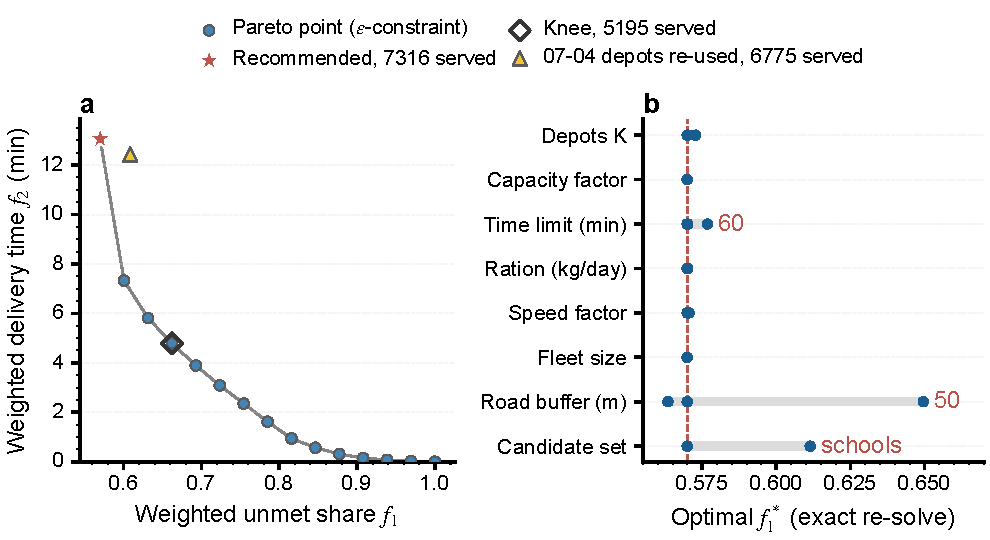
\includegraphics[width=0.98\textwidth,keepaspectratio]{../figures/fig_q5_pareto.pdf}
  \caption{Pareto front and sensitivity of $f_1^*$}
  \label{fig:q5_pareto}
\end{figure}

The front in panel (a) runs from the recommended plan $(f_1,f_2)=(0.570,13.05\ \mathrm{min})$ with 7316 people served to $(1,0)$ with nothing delivered. Its knee lies at $k=3$ with $f_1=0.662$, $f_2=4.79$\,min and 5195 people served: accepting 9 percentage points more unmet need would cut the average delivery time by 63\%. Because the problem stresses serving people in urgent need, we keep the coverage-first plan and report the knee as the alternative if speed matters more, for example for medical supplies.

Measuring the information update takes two solves. Built on the 4 July inputs, the plan opens Xiaoyi, Yunbiao, Liujing, Zhenlong, Hengzhou Town and the Gaocun school, and reaches $f_1=0.477$ under its own inputs. Keeping those depots but re-optimizing shipments against the 16 July cut network and demand gives $f_1=0.609$, $f_2=12.43$\,min and 6775 people served. The value of information is
\begin{equation}
\begin{split}
\mathrm{VoI}_1&=f_1^{04\to16}-f_1^{*,16}=0.609-0.570=0.039,\\
\mathrm{VoI}_2&=f_2^{04\to16}-f_2^{16}\big|_{f_1\le0.609}=12.43-6.89=5.54\ \mathrm{min},
\end{split}
\label{eq:voi}
\end{equation}
i.e. re-planning with the 16 July image lowers the weighted unmet share by 3.9 points, or, at equal coverage, delivers 5.54\,min faster. Read as a two-stage decision, 4 July is the first stage and the 16 July pass is the recourse a real operation would run. A frozen plan then loses at least 3.9 points and 5.5\,min: keeping the first-stage depots and re-optimizing only the shipments already leaves 0.609, the best a stale depot set can do. The tail sits in the depot set itself. Between the two dates the open sets share only half their members (Jaccard 0.50), total demand changes by $-3.57$\,t, and 677 admissible pairs are lost while 625 are gained, because the flood moved. That is the quantity the next satellite pass is worth.

Inputs can also be moved under a frozen plan. Six depots stay fixed and only the shipments are re-optimized -- the recourse an operation would actually run -- while 600 scenarios perturb the demand and the network (Table~\ref{tab:q5_cvar}, Fig.~\ref{fig:q5_cvar}). Demand noise of 20\% (lognormal, truncated at three sigma) moves $f_1$ by nothing, because geometry, not the size of the demand, is the binding constraint. Network noise does cost: cutting each of the 625 pairs that only reopened after 4 July with probability 0.5 gives $f_1=0.604$ and a 5\% quantile of 6345 people served. Over all 600 scenarios $\mathrm{CVaR}_{95}=0.651$; the plan reads as a promise that in 95\% of the futures consistent with the two passes it loses at most eight points of coverage, and in 63\% of them it stays below 0.60. Every reopened pair cut again, the stress case, serves 5846 people at $f_1=0.670$: 20\% fewer than the point estimate, the price of that many roads closing, and the plan never becomes infeasible.

\begin{figure}[H]
  \centering
  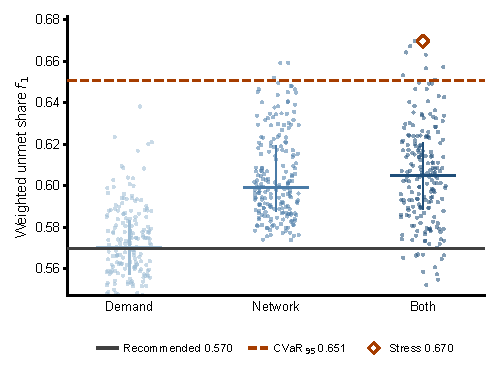
\includegraphics[width=0.86\textwidth,keepaspectratio]{../figures/fig_q5_cvar.pdf}
  \caption{Frozen-plan coverage under 600 scenarios}
  \label{fig:q5_cvar}
\end{figure}

\begin{table}[H]
\centering
\caption{Frozen plan under demand and network uncertainty, 600 scenarios}
\label{tab:q5_cvar}
\small
\begin{tabular}{lrrrr}
\toprule
Scenario family & $f_1$ mean & $f_1$ CVaR$_{95}$ & Served mean & Served $p_{05}$ \\
\midrule
Demand, $\sigma=0.2$ & 0.570 & 0.615 & 7316 & 7316 \\
Network, half of the reopened pairs cut & 0.604 & 0.650 & 6787 & 6345 \\
Both & 0.605 & 0.658 & 6795 & 6468 \\
\midrule
All 600 & 0.593 & 0.651 & 6966 & 6468 \\
Stress, every reopened pair cut & 0.670 & -- & 5846 & -- \\
\bottomrule
\end{tabular}
\end{table}

Panel (b) shows how $f_1^*$ responds to the assumed resources. It is non-increasing in the depot limit, from 0.5728 at $K=3$ to 0.5699 at $K=8$, while the delivery time drops from about 22\,min for $K\le5$ to 9.32\,min at $K=8$. Halving or raising capacity by 50\% leaves $f_1^*=0.5699$; the time limit changes it only at 60\,min (0.5768); the relief norm from 2.5 to 15.6\,kg per person and day changes it by less than 0.0003; a speed factor of 0.6 gives 0.5705, and the fleet size (20, 40 or 60 trucks) has no effect. Only two settings move $f_1^*$ by more than 0.005. The road buffer does: without a buffer $f_1^*=0.564$, with a 50\,m buffer 0.650, because more roads are cut. Restricting the facility proxies to schools alone gives four open depots, $f_1^*=0.611$ and $f_2=21.08$\,min. The plan is therefore robust to the logistic parameters we had to assume and sensitive to the flood extent on the roads, which is the quantity the remote-sensing chain measures.

The allocation is also checked for equity. For every demand unit with at least one admissible pair, a floor $\sum_i x_{ij}\ge q\,d_j$ is added and $q$ scanned from 0 to 1 in steps of 0.2. At the base budget---six depots, 360\,t of capacity against 146.46\,t of demand---nothing moves: $f_1=0.570$, $f_2=13.05$, the reachable unmet share stays zero at every $q$, and the same six depots open. For the 57 units that carry the whole shortfall no admissible pair exists; their gap is geographic, and no allocation rule closes it. Equity here is bounded by geography, not by the objective. The floor binds only when the depot budget is cut: at $K=3$ the base plan already leaves 0.29\% of reachable demand unmet ($f_1=0.573$, $f_2=22.24$, 7237 served) and $q=0.2$ is infeasible. What limits the service floor is therefore the number of staffed sites, not the tonnage: 360\,t covers 146.46\,t with slack, while three depots cannot span the 120-minute catchment. A policy that raises the floor has to add sites, not supplies.

All 19 saved plans (recommended, 4 July, recourse, knee and the 15 front points) were rechecked from the raw inputs with freshly computed shortest paths. Every demand balance closes to within $10^{-6}$\,t, no depot ships more than its capacity or while closed, no plan opens more than six depots, every positive shipment runs on a path within 120\,min that avoids $F$, no open depot lies within 100\,m of new inundation, and the recomputed demands equal the Problem~4 values\cite{deepseek2026,qwen2026,doubao2026}.

% === Letter to the emergency authority (Problem 5) ===
\section[Letter of Recommendations]{Letter of Recommendations to the Hengzhou Emergency Management Bureau}
\label{sec:letter}

\noindent To: Emergency Management Bureau of Hengzhou City, Guangxi\\
From: APMCM Team apmcm26300025\\
Date: 29 November 2026\\
Subject: Using satellite flood maps for relief allocation in Hengzhou

\medskip

Dear Director,

We analyzed the flood around 6 July 2026 in Hengzhou with radar satellite images and public geographic data, and used the results to plan where relief supplies should go\cite{deepseek2026,qwen2026,doubao2026}.

Two radar passes bracket the event. On 4 July, 24.5\,km$^2$ of land that had been dry on 27 June stood under water; on 16 July, 26.9\,km$^2$. That is under one percent of the city, and against the intensity scale we calibrated on labeled flood images it is a ``general'' flood. The percentage is misleading. The water lies in the Yu River valley, where the people and the roads are: about 13,950 residents on flooded ground, 117\,km of road cut, and 75 settlement catchments with no dry route to an unflooded town center or school. Shitang, Maling, Luancheng, Yunbiao, Xiaoyi and Nayang are the worst-hit townships; at village level the catchments of Maling town, Wangzhai, Xinxing, Yangjiang and Xinzhang rank highest.

Monitoring should be radar-first. Optical satellites were blind during the event: no cloud-free scene existed in June, and the nearest one, from 31 May, could not be used. Radar sees through cloud, yet no pass fell between 4 and 16 July, so the peak went unobserved. Two things would help. Request additional radar acquisitions through the emergency satellite tasking channels as soon as a flood warning is issued, and keep one recent dry-season or pre-flood radar image of the whole city on file as the reference for change detection. Before any image is used, check its geolocation against known rivers: ours were displaced by 5.4--6.2\,km and would have produced a wrong map without correction.

Every new pass should trigger a recomputation of the flood map, the catchment ranking and the relief plan; once the data are prepared this takes minutes. A plan made on 4 July and executed on 16 July leaves 3.9 percentage points more priority-weighted need unmet than one re-made with the 16 July image, or, at equal coverage, delivers 5.5 minutes slower on average. Ten days separate the two passes, and half of the depots chosen on 4 July are no longer the best choice; 677 usable depot-to-village connections were lost while 625 new ones opened, and only six of the ten highest-ranked catchments are shared between the two dates. Update after every pass during an event, and publish the map with each update.

For 16 July we recommend opening depots at Taoxu (about 40\,t of supplies over three days), Yunbiao (29\,t), Shitang (5.6\,t), the Gaocun school (2.0\,t), Zhenlong (0.7\,t) and Liujing (0.1\,t), with deliveries routed around flooded roads. This serves about 7300 people within two hours of driving. The remaining 6600 live almost entirely in the 57 affected catchments that no road vehicle can reach within two hours. More stock or more trucks would not help them: raising depot capacity by half, adding 50\% more trucks or extending the delivery limit to four hours left the unserved share almost unchanged. These catchments need boats, high-clearance vehicles or helicopter drops, and supplies pre-positioned before the next flood. Where speed matters more than coverage, for example for medicines, a plan that serves about 5200 people with an average delivery time of 4.8 minutes instead of 13 is available.

Four conditions hold the plan together. Radar data must arrive within a day of acquisition; a few dozen field checks (flood or no flood) should be collected after each event to recalibrate the image model; the Bureau should hold an up-to-date list of township health centers, schools and shelters with their stock and access roads; and the population figures, now from 2020, should be replaced by the current household register. Town centers stood in for facilities here because public data list only five. The relief norm of 3.5\,kg per person per day and the depot capacities are planning values the Bureau should set from its own standards; the plan proved insensitive to both.

As for scope: the method suits river floods on plains and valley floors that radar can observe, such as the Yu River corridor. It is less reliable for flash floods in steep terrain, for floods that rise and fall between two passes, and for water under dense tree canopy or between tall buildings, where radar shadow mimics water and water can hide. On test images the model estimated total flooded area within 1.5\%; for a single small area the error can reach several tens of percent, and in Hengzhou the area moves by up to a factor of two with terrain filters. The intensity grade, the ranking of the most affected areas and the finding that road isolation limits relief held in every check we ran, and those are the results we recommend for decisions.

\medskip

\noindent Yours sincerely,\\
APMCM Team apmcm26300025
\section{Uncertainty Along the Chain and Model Evaluation}
\label{sec:eval}

\subsection{How Assumed Parameters Propagate}

Assumed parameters are varied one at a time; Table~\ref{tab:sens_chain} gives the range and the downstream effect of each.

\begin{table}[!ht]
\centering
\caption{Assumed parameters along the chain}
\label{tab:sens_chain}
\small
\begin{tabular}{p{0.24\textwidth}p{0.17\textwidth}p{0.5\textwidth}}
\toprule
Parameter (problem) & Range tested & Effect \\
\midrule
REM guard $h^*$ (Q3) & 5\,m to none & $A_{new}$ 17.04--40.31\,km$^2$; grade unchanged; Q4 Spearman 0.889 at 30\,m \\
Threshold shift $\Delta\tau$ (Q3) & $-0.2$ to $+0.2$ & $A_{new}$ 1.57--79.52\,km$^2$ over the grid; grade unchanged \\
Change margin $\delta$ (Q3) & 0--4.5\,dB & $A_{new}$ 32.40--23.59\,km$^2$ \\
$W_0$ definition (Q3) & union / SAR$+$WC / SAR only & $A_{new}$ 26.90 / 27.29 / 30.47\,km$^2$; Q4 Spearman 0.996 (WC) / 0.932 (SAR only) \\
SAR scale (Q3) & dB / amplitude & 26.90 / 49.39\,km$^2$; dB chosen by KS distance 0.106 vs 0.241 \\
Indicator weights (Q4) & Dirichlet ($M{=}2000$) & median Spearman 0.987, 5\% quantile 0.934 \\
Depot limit $K$ (Q5) & 3--8 & $f_1^*$ 0.5728--0.5699; $f_2$ about 22 to 9.32\,min \\
Capacity, fleet, $T_{max}\ge90$, $q$ (Q5) & $\times0.5$--$1.5$; 20--60; 90--240\,min; 2.5--15.6\,kg & $f_1^*$ changes by at most 0.0003 \\
Road buffer (Q5) & 0 / 20 / 50\,m & $f_1^*$ 0.564 / 0.570 / 0.650 \\
\bottomrule
\end{tabular}
\end{table}

Area moves with terrain and thresholds, 1.57--79.52\,km$^2$ over the grid; decisions do not. The grade stays ``general'', the 16 July ranking keeps Spearman at least 0.889, and the plan moves only with flooded roads, 0.564 without a buffer against 0.650 at 50\,m.

\subsection{Strengths and Innovations}

Every number is held out: validation is spatially blocked, calibration folds are kept separate, and leave-one-cluster-out leaves IoU 0.508. One raster $F$ supplies hazard, cut network, demand and priority, and the MILP closes with zero gap. The mask is cut at the calibrated area \eqref{eq:tauA}, not at 0.5 or the F1 optimum, with a conformal interval on every tile; grades are probability vectors \eqref{eq:grade_mc}; and a second satellite pass is worth 3.9 points of unmet share.

\subsection{Conclusions}

One chain runs from images to relief. LightGBM reaches IoU 0.618 at $-0.2\%$ after the 50\,px MMU; the gated U-Net reaches 0.797 at $+0.9\%$ in-domain and 0.730 at $+1.45\%$ after transfer. Grades split at 5.9\%, 53.0\% and 96.9\%. In Hengzhou 16 July gives 26.90\,km$^2$ new, 0.78\% of the city and grade ``general'', with a net $-52.53$\,km$^2$ from receding water. On 393 catchments Shitang, Maling and Luancheng rank highest, stable under weight perturbation. The MILP opens six depots and serves 7316 of 13,948; the rest is cut off by water, so the shortfall is a floor, not slack. Across 600 scenarios CVaR$_{95}$ is 0.651 and the plan stays feasible\cite{deepseek2026,qwen2026,doubao2026}.


% === References ===
% References start on a fresh page (section XI); entries are hand-written in
% references.tex so that every item carries the APMCM type code and full fields
\clearpage
% References in the APMCM-required format:
%   [ID] author, title[type], source, year, volume(issue), pages
%   online resources: [ID] author, title[EB/OL], web site, visit time
% Type codes: [J] journal, [C] conference proceedings, [CP/OL] computer program,
% [EB/OL] electronic resource. Entries are ordered by first citation.

\begin{thebibliography}{20}

\bibitem{deepseek2026}
DeepSeek. DeepSeek-V4-Flash[EB/OL]. Hangzhou DeepSeek Artificial Intelligence Basic Technology Research Co., Ltd., \url{https://www.deepseek.com}, 2026-11-27.

\bibitem{qwen2026}
Tongyi Qianwen (Qwen). Qwen3.8-Max[EB/OL]. Alibaba Cloud Computing Co., Ltd., \url{https://tongyi.aliyun.com}, 2026-11-27.

\bibitem{doubao2026}
Doubao. Doubao 2.0 Pro[EB/OL]. Beijing Douyin Information Service Co., Ltd., \url{https://www.doubao.com}, 2026-11-27.

\bibitem{martinis2009splitbased}
S. Martinis, A. Twele, S. Voigt. Towards operational near real-time flood detection using a split-based automatic thresholding procedure on high-resolution TerraSAR-X data[J]. Natural Hazards and Earth System Sciences, 2009, 9(2): 303-314.

\bibitem{twele2016sentinel1}
A. Twele, W. Cao, S. Plank, S. Martinis. Sentinel-1-based flood mapping: a fully automated processing chain[J]. International Journal of Remote Sensing, 2016, 37(13): 2990-3004.

\bibitem{ronneberger2015unet}
O. Ronneberger, P. Fischer, T. Brox. U-Net: convolutional networks for biomedical image segmentation[C]//Proceedings of the 18th International Conference on Medical Image Computing and Computer-Assisted Intervention (MICCAI 2015). Cham: Springer, 2015: 234-241.

\bibitem{bonafilia2020sen1floods11}
D. Bonafilia, B. Tellman, T. Anderson, E. Issenberg. Sen1Floods11: a georeferenced dataset to train and test deep learning flood algorithms for Sentinel-1[C]//2020 IEEE/CVF Conference on Computer Vision and Pattern Recognition Workshops (CVPRW). Piscataway: IEEE, 2020: 835-845.

\bibitem{nobre2011hand}
A. D. Nobre, L. A. Cuartas, M. Hodnett, et al. Height above the nearest drainage -- a hydrologically relevant new terrain model[J]. Journal of Hydrology, 2011, 404(1-2): 13-29.

\bibitem{balcik2008facility}
B. Balcik, B. M. Beamon. Facility location in humanitarian relief[J]. International Journal of Logistics Research and Applications, 2008, 11(2): 101-121.

\bibitem{mcfeeters1996ndwi}
S. K. McFeeters. The use of the normalized difference water index (NDWI) in the delineation of open water features[J]. International Journal of Remote Sensing, 1996, 17(7): 1425-1432.

\bibitem{lee1980local}
J.-S. Lee. Digital image enhancement and noise filtering by use of local statistics[J]. IEEE Transactions on Pattern Analysis and Machine Intelligence, 1980, PAMI-2(2): 165-168.

\bibitem{roberts2017crossvalidation}
D. R. Roberts, V. Bahn, S. Ciuti, et al. Cross-validation strategies for data with temporal, spatial, hierarchical, or phylogenetic structure[J]. Ecography, 2017, 40(8): 913-929.

\bibitem{lightgbm2020package}
Y. Shi, G. Ke, D. Soukhavong, et al. lightgbm: light gradient boosting machine[CP/OL]. The R Foundation, \url{https://doi.org/10.32614/CRAN.package.lightgbm}, 2020-09 [2026-11-27].

\bibitem{bland1986agreement}
J. M. Bland, D. G. Altman. Statistical methods for assessing agreement between two methods of clinical measurement[J]. The Lancet, 1986, 327(8476): 307-310.

\bibitem{lundberg2020trees}
S. M. Lundberg, G. Erion, H. Chen, et al. From local explanations to global understanding with explainable AI for trees[J]. Nature Machine Intelligence, 2020, 2(1): 56-67.

\bibitem{lin2017focal}
T.-Y. Lin, P. Goyal, R. Girshick, et al. Focal loss for dense object detection[C]//2017 IEEE International Conference on Computer Vision (ICCV). Piscataway: IEEE, 2017: 2999-3007.

\bibitem{zadrozny2002calibration}
B. Zadrozny, C. Elkan. Transforming classifier scores into accurate multiclass probability estimates[C]//Proceedings of the 8th ACM SIGKDD International Conference on Knowledge Discovery and Data Mining. New York: ACM, 2002: 694-699.

\bibitem{lei2018conformal}
J. Lei, M. G'Sell, A. Rinaldo, et al. Distribution-free predictive inference for regression[J]. Journal of the American Statistical Association, 2018, 113(523): 1094-1111.

\bibitem{diakoulaki1995critic}
D. Diakoulaki, G. Mavrotas, L. Papayannakis. Determining objective weights in multiple criteria problems: the CRITIC method[J]. Computers \& Operations Research, 1995, 22(7): 763-770.

\bibitem{huangfu2018highs}
Q. Huangfu, J. A. J. Hall. Parallelizing the dual revised simplex method[J]. Mathematical Programming Computation, 2018, 10(1): 119-142.

\end{thebibliography}


% === AI 工具使用声明（紧随参考文献）===
% 由 build_ai_disclosure.py 根据用户确认记录生成，请勿由模型改写。
\clearpage
\section*{Report on Use of AI}
Our team used AI tools in this competition, as follows:

1. DeepSeek (DeepSeek-V4-Flash), used on 2026-11-26, for language polishing; code debugging.

2. 通义千问（Qwen） (Qwen3.8-Max), used on 2026-11-26, for language polishing; typesetting checks; terminology checking; code debugging; reference formatting.

3. 豆包 (豆包 2.0 Pro), used on 2026-11-26, for language polishing; typesetting checks; terminology checking.

4. Claude (claude-opus-5-5, Anthropic), used on 2026-11-26, for problem analysis; modeling and solution; coding; generating the data figures; drafting the paper.


% === Appendix ===
\begin{appendices}
% 附录小节号跟随附录字母（A.1、A.2 …），与目录和标题一致
\renewcommand\thesubsection{\thesection.\arabic{subsection}}
% 编号 A. 已表明附录，目录条目不再重复 “Appendix” 一词
\renewcommand{\appendixname}{}
\section{Key Algorithm Code}

The complete, runnable code is organized as \texttt{config.py} (all parameters), \texttt{common.py} (pixel area, normalization, Lee filter, indices and features), \texttt{problem1.py} to \texttt{problem5.py}, \texttt{unet.py} and an independent audit script for the relief plans; \texttt{main.py} runs the chain. The excerpts below are the core routines referred to in the paper.

\subsection{Gated fusion network and area-consistent loss}

\begin{lstlisting}[language=Python]
class GatedFusionUNet(nn.Module):
    """SAR branch + optional optical branch; at each scale s the fused feature is
    h = g*h_S + (1-g)*h_O with g = sigmoid(W_g * [h_S; h_O]) (1x1 conv)."""
    def forward(self, x_sar, x_opt=None, return_gates=False):
        hs = self.enc_s(x_sar)
        if self.use_opt:
            ho = self.enc_o(x_opt)
            skips, gvals = [], []
            for s, gate in enumerate(self.gates):
                g = torch.sigmoid(gate(torch.cat([hs[s], ho[s]], 1)))
                skips.append(g * hs[s] + (1 - g) * ho[s])
                gvals.append(g.mean())
        else:
            skips, gvals = hs, []
        x = self.drop(self.bott(F.max_pool2d(skips[-1], 2)))
        for d, skip in zip(self.dec, reversed(skips)):
            x = F.interpolate(x, size=skip.shape[-2:], mode="bilinear", align_corners=False)
            x = self.drop(d(torch.cat([x, skip], 1)))
        out = self.head(x)[:, 0]
        return (out, gvals) if return_gates else out

def flood_loss(logit, y, valid, lam_area=1.0, gamma=2.0, alpha1=0.75):
    """Focal + soft Dice + lambda_A * area consistency, valid pixels only."""
    v = valid.float(); p = torch.sigmoid(logit); yf = y.float()
    pt = torch.where(yf > 0.5, p, 1 - p).clamp(1e-6, 1 - 1e-6)
    at = torch.where(yf > 0.5, torch.full_like(p, alpha1), torch.full_like(p, 1 - alpha1))
    focal = (-(at * (1 - pt) ** gamma * torch.log(pt)) * v).sum() / v.sum().clamp(min=1)
    inter = (p * yf * v).sum()
    dice = 1 - (2 * inter + 1) / ((p * v).sum() + (yf * v).sum() + 1)
    nb = v.sum((1, 2)).clamp(min=1)
    area = (((p - yf) * v).sum((1, 2)).abs() / nb).mean()
    return focal + dice + lam_area * area
\end{lstlisting}

\subsection{Area-preserving threshold}

\begin{lstlisting}[language=Python]
def area_preserving_tau(pbar, wA, expected, lo=0.01, hi=0.99, tol=1e-4):
    """bisection: sum a*1[p>=tau] = sum a*q(p); left side non-increasing in tau."""
    def f(t):
        return float((wA * (pbar >= t)).sum()) - expected
    if f(lo) < 0 or f(hi) > 0:
        lo, hi = 0.001, 0.999
    while hi - lo > tol:
        mid = 0.5 * (lo + hi)
        if f(mid) > 0:
            lo = mid
        else:
            hi = mid
    t = lo if abs(f(lo)) <= abs(f(hi)) else hi
    return t, f(t) + expected
\end{lstlisting}

\subsection{Grade thresholds and grade probabilities}

\begin{lstlisting}[language=Python]
def gmm_thresholds(x, seed=2026, n_init=20, K=4):
    """Bayes boundaries between adjacent components of a K-component 1-D GMM on logit(rho)."""
    g = GaussianMixture(n_components=K, covariance_type="full", n_init=n_init,
                        random_state=seed).fit(x[:, None])
    order = np.argsort(g.means_.ravel())
    mu = g.means_.ravel()[order]; sd = np.sqrt(g.covariances_.ravel()[order]); pi = g.weights_[order]
    th = []
    for j in range(K - 1):
        fun = lambda t: (np.log(pi[j]) + norm.logpdf(t, mu[j], sd[j])
                         - np.log(pi[j + 1]) - norm.logpdf(t, mu[j + 1], sd[j + 1]))
        a, b = mu[j], mu[j + 1]
        if not (fun(a) > 0 and fun(b) < 0):
            return None, dict(mu=mu, sd=sd, pi=pi)
        th.append(brentq(fun, a, b))
    theta = 1 / (1 + np.exp(-np.array(th)))
    ok = bool(np.all(np.diff(theta) > 0) and theta[0] > 0 and theta[-1] < 1)
    return (theta if ok else None), dict(mu=mu, sd=sd, pi=pi, bic=g.bic(x[:, None]))

def mc_grades(Ahat, sigp, Areg, resid_pool, boot_theta, M=2000, seed=2026):
    """grade probabilities pi_jg for units j (one shared residual per draw)."""
    rng = np.random.default_rng(seed)
    r = rng.choice(resid_pool, M, replace=True)
    th = boot_theta[rng.integers(0, len(boot_theta), M)]
    A = np.clip(Ahat[:, None] + r[None, :] * sigp[:, None], 0, Areg[:, None])
    rho = A / Areg[:, None]
    g = 1 + (rho[:, :, None] >= th[None, :, :]).sum(2)
    return np.stack([(g == gg).mean(1) for gg in (1, 2, 3, 4)], 1)
\end{lstlisting}

\subsection{Guarded newly inundated set in Hengzhou}

\begin{lstlisting}[language=Python]
def compute_F(meta, date, tauA, dtau=0.0, hstar=15.0, delta=3.0, w0mode="union", mmu=50, scale="db"):
    """F_d = MMU( {p>=tau_A+dtau} & ~W0 & {REM<=h*} & {dVV<=-delta} ) inside the boundary."""
    # ... memory-mapped rasters: PB (mean probability), W0, boundary bm, Lee-filtered VV, REM ...
    for r in range(0, Hh, 512):
        sl = slice(r, min(r + 512, Hh))
        raw = (PB[sl] >= tauA + dtau) & (bm[sl] > 0)
        c1 = raw & (W0[sl] == 0)                                   # not pre-flood water
        rem = rem10_strip(rem30, r, sl.stop - r, Ww)
        c2 = c1 & (np.nan_to_num(rem, nan=1e9) <= hstar)           # REM guard
        dvv = np.nan_to_num(lf_d[sl] - lf_0[sl], nan=0.0)
        cand[sl] = c2 & (dvv <= -delta)                            # change guard
    return U.mmu_filter(cand, mmu) if mmu > 1 else cand            # minimum mapping unit
\end{lstlisting}

\subsection{Depot-activation and allocation MILP}

\begin{lstlisting}[language=Python]
def build(obj):
    m = pulp.LpProblem("relief", pulp.LpMinimize)
    eta = {i: pulp.LpVariable(f"eta_{i}", cat=pulp.LpBinary) for i in range(nI)}
    f = {(i, j): pulp.LpVariable(f"f_{i}_{j}", lowBound=0) for (i, j) in A}
    u = {j: pulp.LpVariable(f"u_{j}", lowBound=0) for j in range(nJ)}
    f1 = pulp.lpSum(w[j] * u[j] for j in range(nJ)) * (1.0 / Wd)
    f2 = pulp.lpSum(w[j] * tt[i, j] * f[i, j] for (i, j) in A) * (1.0 / Wd)
    for j in range(nJ):                                   # demand balance
        m += pulp.lpSum(byj.get(j, [])) + u[j] == d[j]
    for i in range(nI):                                   # capacity, open depots only
        m += pulp.lpSum(byi.get(i, [])) <= cap[i] * eta[i]
        if not cand["admissible"].iloc[i]:               # depots near F stay closed
            m += eta[i] == 0
    for (i, j) in A:                                      # valid tightening
        m += f[i, j] <= d[j] * eta[i]
    m += pulp.lpSum(eta.values()) <= p["K"]               # at most K open depots
    m += pulp.lpSum((2 * tt[i, j] + p["t_load"]) / p["q_veh"] * f[i, j] for (i, j) in A) \
        <= 60 * p["n_veh"] * p["shift"] * p["H"]          # fleet vehicle-minutes
    return m, eta, f, u, f1, f2
# lexicographic: min f1, then min f2 s.t. f1 <= f1* + 1e-6; HiGHS with gapRel = 0
\end{lstlisting}

\end{appendices}

\end{document}
